\section{The functional renormalization group}\label{sec:FRG}
The \acrrepeat{frg}~\cite{\frgWetterichEq} and \dses{}~\cite{Dyson:1949ha,Schwinger:1951ex,Schwinger:1951hq} are two major functional methods used to study \qfts{}.
Related \tpi{} and \npi{} techniques, see, \eg{}, \ccite{Berges:2004pu,Berges:2005hc,Pawlowski:2005xe,Carrington:2010qq,Blaizot:2021ikl} as well as the lecture notes~\cite{Berges:2004yj}, are also popular for certain applications.
Those functional methods are used to compute correlation functions (or their generating functionals) using non-perturbative loop equations.

Within this work we will primarily work with the \frg{} which we will introduce on a technical level in the following subsections. For more details we refer the interested reader to the lecture notes~\cite{Berges:2000ew,PawlowskiScript,Gies:2006wv,Kopietz:2010zz} as well as to the following \ccite{Wetterich:2001kra,Pawlowski:2005xe,Rosten:2010vm,Delamotte:2007pf,Dupuis:2020fhh}.
For details regarding \dses{}, see, \eg{}, \ccite{Fischer:2018sdj} and references therein.
The \frg{} was developed in the early 1990s by Christof Wetterich~\cite{\frgWetterichEqA} and others, including notable early developments by Martin Reuter, Tim R. Morris, Nikolaos Tetradis, and Ulrich Ellwanger~\cite{\frgWetterichEqB}.\bigskip\FloatBarrier

\begin{figure}[!t]
\begin{center}%
	\vspace{-0.5em}\includegraphics{frg/figures/frg_flow.pdf}%
\end{center}%
	\caption{%
		Sketch of the \acrshort{frg} flow of the \acrshort{eaa} $\FSeaa_k[\FSsf]$ from its initial condition $S_\Lambda[\FSsf]$ in the \acrshort{uv} ($k=\Lambda$) towards the full quantum \acrshort{ea} in the \acrshort{ir} ($k\rightarrow 0$).%
	}%
	\label{fig:rg_scetch}%
\end{figure}%
Before a discussion of the \frg{} on a technical level (culminating in the derivation and discussion of the central \frgEquation{} in \cref{subsec:wetterich}), we will outline the idea behind this powerful non-perturbative method.
The \frg{} implements Kenneth G. Wilson's non-perturbative continuum \rg{} approach~\cite{Wilson:1971bg,Wilson:1971dh,Wilson:1979qg} in momentum space and thus by extension the discrete equivalent \dash{} position space based \dash{} \rg{} concept of Leo P. Kadanoff's block-spin transformations~\cite{Kadanoff:1966wm}.
The conceptual idea behind the \rg{} is the study of physical systems/theories at different scales.
The \grg \footnote{%
	We use \acrshort{grg} when making statements which apply for the functional renormalization group as well as for the non-perturbative renormalization group in general.%
} can be used to study the scale evolution of a theory from a microscopic scale \dash{} where the theory is initially defined using microscopic interactions \dash{} to a macroscopic scale \dash{} where we can compute macroscopic observables and correlation functions of the physical system under consideration.
The changes during scale evolution in the correlation functions and observables of a field theory are governed by quantum and/or thermodynamic fluctuations.
Considering a functional formulation of \qft{} based on a suitable functional integral, Wilson's \rg{} approach is based on integrating out fluctuations step by step \dash{} momentum shell by momentum shell.
This incremental study of successive \rg{} steps facilitates the practical computation of the underlying functional integral, which is usually not possible when trying to incorporate all fluctuations at once.

The \frg{} describes the \rgscaleevolution{} of a scale-dependent \eaa{} $\FSeaa_k[\FSsf]$ as a series of infinitesimal \rg{} steps in form of a so-called \rg{} flow.
See \cref{fig:rg_scetch} for a pictographic sketch of this process.
In the following we use $k$ to denote the \rgscale{}.
The starting point of the \frg{} flow is $\FSeaa_\Lambda[\FSsf]$ which is based on an Euclidean action $S_\Lambda[\FSsf]$ at a \rg{} \uv{} initial scale $k=\Lambda$.
The action at this scale is considered ``classical'' in a sense that either $\Lambda$ is asymptotically large or $S_\Lambda[\FSsf]$ includes all quantum fluctuations with momenta $|p|>\Lambda$.
Starting at the initial scale $\Lambda$ the idea is to integrate out fluctuations successively in a Wilsonian manner by splitting the quantum fields based on their momenta.
In the \frg{} this is achieved by introducing a suitable regulator which ultimately implements and facilitates this process.
The \rgscaleevolution{} in the \frg{} is governed by one central non-perturbative one-loop equation \dash{} the so-called \textit{Wetterich} flow equation~\cite{\frgWetterichEq}.
This non-linear functional differential equation is exact given a suitable regulator choice and thus maps the problem of solving the functional integral to solving a corresponding flow equation.
Using this flow equation, one can track the change of a microscopic theory with a given action $\FSeaa_\Lambda[\FSsf]=S_\Lambda[\FSsf]$ in the \uv{} ($k=\Lambda$) towards a macroscopic theory with a full quantum effective action $\FSeaa_0[\FSsf]=\Gamma_\mathrm{1PI}[\FSsf]$ in the \ir{}~(${k\rightarrow 0}$).
The \frg{} is inherently non-perturbative and thus allows the study of both weakly and strongly coupled systems.
Using the scale-dependent \eaa{} $\FSeaa_k[\FSsf]$ it is in principle possible to study the ground state, realized symmetries, thermodynamic properties, and correlation functions of a theory at varying  \rgscales{} $k$. 
This makes the \frg{} an immensely powerful tool to study the effect of quantum and/or thermodynamic fluctuations in a wide range of physical systems at different scales in a controlled and unified framework.

\subsection{Scale-dependent generating functionals}\label{subsubsec:generatingFunctionals}
We begin our technical discussion of the \frg{} by introducing two auxiliary scale-dependent generating functionals.

For the following discussion we consider a quantum field theory with the Euclidean action $\Sinit[\FSff{\FSsf}]$, where $\FSff{\FSsf}$ is a multi component fundamental quantum field which includes the entire field content of the theory under consideration in the \fs{} notation of \cref{app:FS}.
In the subsequent derivation we consider a generic theory in which $\FSff{\FSsf}$ collects scalar (mesonic) fields $\FSff{\MFphi}$ and Grassmann-valued (fermionic) fields $\FSff{\MFpsi}$ and $\FSff{\MFpsib}$:
\begin{align}
	(\FSffd{\FSsf}{a})\equiv (\FSff{\MFphi},\FSff{\MFpsi},\FSff{\MFpsib})\,.
\end{align}

We further introduce $\FSf{\FSsf}$ as a \rgscaledependent{} multi component composite field of the fundamental fields
\begin{align}
	(\FSfd{\FSsf}{a})\equiv (\FSf{\FSsf}_{k;\FSidx{a}}[\FSff{\FSsf}])\,.
\end{align}
For readability we will usually suppress the scale and functional dependency in the notation.
We introduce corresponding sources
\begin{align}
	(\FSfd{J}{a})\equiv (\FSf{J}_{\MFphi},\FSf{J}_{\MFpsib}, \FSf{J}_{\MFpsi})
\end{align}
in the generating functional to extract correlation functions and to study condensation.
Working with such scale-dependent composite fields as degrees of freedom is more elegant and efficient since the fundamental fields of a theory are not necessary suitable degrees of freedom at all scales.
A prime example for this is \qcd{}, where the fundamental fields are quarks and gauge fields which are excellent degrees of freedom in the \uv{} (at some \uv{} reference scale $\Lambda$) due to asymptotic freedom.
In the \ir{} ($k\rightarrow0$) however \dash{} due to confinement and chiral symmetry breaking \dash{} a description in terms of hadrons is desirable, since baryons and mesons are the relevant degrees of freedom.
Introducing those hadrons as composite fields of the fundamental fields has proven highly effective and elegant in \frg{} studies of \qcd{}, see, \eg{}, \ccite{Alkofer:2018guy,Fu:2019hdw,Fu:2022gou} and references therein and \cref{subsec:chiralLEFT}.

To implement Wilson's \rg{} approach we introduce a \rgscaledependent{} regulator term $\Delta S_k[\FSf{\FSsf}]$ in the Euclidean generating functional of the theory under consideration
\begin{align}
	Z_k[\FSf{J}]=\exp\del[3]{-\Delta S_k\sbr{\frac{\delta}{\delta \FSf{J}}}}Z[\FSf{J}]= \int \mathcal{D}[\FSff{\FSsf}] \exp\del{-\Sinit[\FSff{\FSsf}]-\Delta S_k[ \FSf{\FSsf}]+\FSfu{J}{m}\FSfd{\FSsf}{m}}\,,
	\label{eq:ZkDef}
\end{align}
where $\Sinit[\FSff{\FSsf}]$ is the Euclidean, classical action prescribing kinematics and interactions of the fundamental fields $\FSff{\FSsf}$. 
$\mathcal{D}[\FSff{\FSsf}]$ is a suitable functional integral measure including a possible normalization factor $\mathcal{N}$ and appropriate boundary conditions for the fields when working at non-zero temperature, see \cref{app:thermalQFT} for details.
Such a normalization factor $\mathcal{N}$ is arbitrary, since it does not affect observables and thus varies depending on the conventions used for $Z[\FSf{J}]$.
General expectation values in presence of $\FSf{J}$ and $\Delta S_k[\FSf{\FSsf}]$  are given by
\begin{align}
	\expectationValue{O[\FSf{\FSsf}]}{\FSf{J}} =\frac{1}{Z_k[\FSf{J}]}  \int \mathcal{D}[\FSff{\FSsf}]\, O[\FSf{\FSsf}] \exp\del{-\Sinit[\FSff{\FSsf}]-\Delta S_k[ \FSf{\FSsf}]+\FSfu{J}{m}\FSfd{\FSsf}{m}}
	\label{eq:expectationOJ}\,.
\end{align}
From \cref{eq:expectationOJ} one obtains the useful identity
\begin{align}
	\frac{\delta}{\delta \FSfu{J}{a}}\expectationValue{O[\FSf{\FSsf}]}{\FSf{J}} = -\expectationValue{\FSfd{\FSsf}{a}}{\FSf{J}}\expectationValue{O[\FSf{\FSsf}]}{\FSf{J}} + \expectationValue{\FSfd{\FSsf}{a}O[\FSf{\FSsf}]}{\FSf{J}}
	\label{eq:dexpectationOJdJ}\,.
\end{align}
For practical computations in the scope of this work it is convenient to choose a regulator term $\Delta S_k[ \FSf{\FSsf}]$ which  is quadratic in the fields
\begin{align}
	\Delta S_k[ \FSf{\FSsf}] 
	\equiv  \Delta S[ \FSf{\FSsf},R_k]
	\equiv \frac{1}{2} \FSregulator{\FSidx{m},\FSidx{n}}\FSfd{\FSsf}{n}\FSfd{\FSsf}{m}\,,\label{eq:DeltaSRab}
\end{align}
where we introduced the regulator $\FSregulator{\FSidx{m},\FSidx{n}}$\footnote{%
	We have chosen $\frac{1}{2} \FSregulator{\FSidx{m},\FSidx{n}}\FSfd{\FSsf}{n}\FSfd{\FSsf}{m}$ and not $\FSregulator{\FSidx{n},\FSidx{m}}\FSfd{\FSsf}{n}\FSfd{\FSsf}{m}$ like in \ccite{Pawlowski:2005xe} out of personal preference especially related to the form of \cref{eq:DeltaSab}.%
}.
$\Delta S_k[ \FSf{\FSsf}] $ should appear as a scalar in the exponent under the functional integral. This implies a bilinear form of the regulator for Grassmann-valued FS components with 
\begin{align}
	\FSregulator{\FSidx{m},\FSidx{n}} = \FSc{\FSidx{n},\FSidx{m}} \FSregulator{\FSidx{n},\FSidx{m}}
\end{align}
and a non-trivial structure in its internal spaces. A quadratic regulator leads to one-loop flow equations for all \nptFunctions{}~\cite{Litim:2002xm,Pawlowski:2005xe}.
Higher-order regulators are possible, see, \eg{}, \ccite{Pawlowski:2005xe}, but will not be discussed in our work.
With the definition \eqref{eq:DeltaSRab} the second FS derivative of the regulator term is given by
\begin{align}
	\Delta S[ \FSf{\FSsf},R_k]_{,\FSidx{a}\FSidx{b}}
	=\frac{1}{2} \frac{\delta}{\delta \FSfd{\FSsf}{a}}\frac{\delta}{\delta \FSfd{\FSsf}{b}}\FSregulator{\FSidx{m},\FSidx{n}}\FSfd{\FSsf}{n}\FSfd{\FSsf}{m}
	=\frac{1}{2} \frac{\delta}{\delta \FSfd{\FSsf}{a}}\del{
	\FSregulator{\FSidx{m},\FSidx{b}}\FSfd{\FSsf}{m}+\FSc{\FSidx{b},\FSidx{n}}\FSregulator{\FSidx{b},\FSidx{n}}\FSfd{\FSsf}{n}
	}
	=\FSregulator{\FSidx{a},\FSidx{b}}\,.\label{eq:DeltaSab}
\end{align}
We will discuss further constraints on the regulator related to the proper implementation of Wilson's \rg{} approach in \cref{subsubsec:regulator}.

The scale-dependent Schwinger functional $W_k[\FSf{J}]$ is given by 
\begin{align}
	W_k[\FSf{J}] = \ln Z_k[\FSf{J}]\,.\label{eq:WkDef}
\end{align}
Considering functional derivatives of the Schwinger functional leads to connected \nptFunctions{}, see, \eg{}, \ccite{Iliopoulos:1974ur,ZinnJustin:2002ru,Weinberg:1996kr,Peskin:1995ev,PawlowskiScript}. The one-point function \dash{} the expectation value of $\FSf{\FSsf}$ in presence of $\Delta S_k[ \FSf{\FSsf}]$ and $\FSf{J}$ \dash{} is simply given by
\begin{align}
	\frac{\delta}{\delta \FSfu{J}{a}}W_k[\FSf{J}] = \frac{1}{Z_k[\FSf{J}]}\frac{\delta Z_k[\FSf{J}]}{\delta\FSfu{J}{a}}=\expectationValue{\FSfd{\FSsf}{a}}{\FSf{J}}\,.\label{eq:dWkdJa}
\end{align}
To study the \rgscale{} evolution of $W_k[\FSf{J}]$ and by extension $Z_k[\FSf{J}]$ we consider the total \rg-scale derivative\footnote{%
	Total derivatives \wrt{} the \acrshort{rg} scale (\acrshort{rg} time) will be frequently abbreviated by $\partial_k$ ($\partial_t$) in the following.
	We denote \acrshort{rg} scale-dependence with either $k$ or $t$ depending on the element and context.
	In terms of derivatives both are always understood as $k(t)$ and $t(k)$.
	The reasoning behind this mixed use of $k$ and $t$ in formulas is that for the discussion of flow/evolution we like $t$ while for denoting \acrshort{ir} and \acrshort{uv} we prefer $k$.%
} of $W_k[\FSf{J}]$.
It is convenient to study and discuss the scale evolution from $k=\Lambda$ to $k\rightarrow0$ using a dimensionless \rg/flow time $t$ which we define\footnote{%
	We adopt a sign convention for the \rg{} flow time resulting in a positive time evolution from the \uv{} ($k=\Lambda\Leftrightarrow t=0$) to the \ir{} ($k \rightarrow 0 \Leftrightarrow t\rightarrow \infty$).
} as
\begin{align}
	&t \equiv - \ln \big( \tfrac{k}{\Lambda} \big) =  \ln \big( \tfrac{\Lambda}{k} \big) \, ,	\qquad	t \in [ 0, \infty ) \, .	\label{eq:def_rg_time}
\end{align}
The evolution equation for $W_k[\FSf{J}]$ is given by
\begin{align}
	\stepcounter{equation}\newSubEqBlock
	\dod{W_k[\FSf{J}]}{t}&=\dod{}{t}\ln Z_k[\FSf{J}]
	=\frac{1}{Z_k[\FSf{J}]}\dod{Z_k[\FSf{J}]}{t}\, = \subEqTag\\
	&=\frac{1}{Z_k[\FSf{J}]} \int \mathcal{D}[\FSff{\FSsf}]\, \dod{}{t}\exp\del{ -\Sinit[\FSff{\FSsf}] - \frac{1}{2} \FSregulator{\FSidx{m},\FSidx{n}}\FSfd{\FSsf}{n}\FSfd{\FSsf}{m} +\FSfu{J}{m}\FSfd{\FSsf}{m} }\, = \subEqTag\\
	&= \FSfu{J}{m}\expectationValue{\partial_t \FSfd{\FSsf}{m}}{\FSf{J}}-\frac{1}{2}\del{\partial_t \FSregulator{\FSidx{m},\FSidx{n}}}\expectationValue{\FSfd{\FSsf}{n}\FSfd{\FSsf}{m}}{\FSf{J}}- \FSregulator{\FSidx{m},\FSidx{n}}\expectationValue{\FSfd{\FSsf}{n}\partial_t\FSfd{\FSsf}{m}}{\FSf{J}}\label{eq:dWkdt},
\end{align}
where we considered $k=k(t)\equiv\Lambda\,\eu^{-t}$.
\Cref{eq:dWkdt} is the generalization of the Polchinski equation~\cite{Polchinski:1983gv} for composite fields with \ir{} regularization~\cite{PawlowskiScript}\footnote{%
	However, in the original work~\cite{Polchinski:1983gv} an effective action $L ( \Lambda, \phi )$ takes the role of $W_k[\FSf{J}]$ and it is formulated in terms of the fields $\phi$ instead of the sources $\FSf{J}$. For relations between the original Polchinski equation and the flow equations studied in this work and selected applications of the Polchinski equation, see, \eg{}, \ccite{Litim:2005us,Yabunaka:2018mju,Litim:2018pxe,Cotler:2022fze,Fu:2022gou}.
}.
We will discuss the scale-dependent Schwinger functional further in \cref{subsubsec:WtJd0} in the context of zero-dimensional \qfts{}.

\subsection{Scale-dependent effective average action}\label{subsec:frgeaa}
While working with \rg{} equations \eqref{eq:dWkdt} for the Schwinger functional is possible, it is more convenient for most practical computations to work with the scale-dependent \eaa{} $\FSeaa_k[\FSmf{\FSsf}]$  which is given by the modified Legendre transform of the Schwinger functional
\begin{align}
	\FSeaa_k[\FSmf{\FSsf}]&\equiv\FSea_k[\FSmf{\FSsf}] -\Delta S_k[\FSmf{\FSsf}] \equiv\sup_{\FSf{J}}\del{
	\FSfu{J}{m}\FSmfd{\FSsf}{m}-W_k[\FSf{J}]
	}-\Delta S_k[\FSmf{\FSsf}] \label{eq:Gammaksup}\, , \\
	\FSeaa_k[\FSmf{\FSsf}]+\Delta S_k[\FSmf{\FSsf}] &= \FSea_k[\FSmf{\FSsf}] = \FSmfu{J}{m}\FSmfd{\FSsf}{m}-W_k[\FSmf{J}]\, ,\label{eq:Gammak}
\end{align}
where we denote $\FSmfu{J}{m}$ as the source $\FSfu{J}{m}$ which realizes the supremum for a given so-called mean-field $\FSmfd{\FSsf}{m}$ and $\Delta S_k[\FSmf{\FSsf}]=\FSregulator{\FSidx{m},\FSidx{n}}\FSmfd{\FSsf}{n}\FSmfd{\FSsf}{m}/2$ in analogy to \cref{eq:DeltaSRab}.
The modification of the Legendre transform with $\Delta S_k[\FSmf{\FSsf}]$ is necessary in order to implement $\FSeaa_k\rightarrow S_\Lambda$ in the \uv{} limit $k\rightarrow \Lambda$, see \cref{subsubsec:zerodICS} for a detailed discussion of this subtle point. 
$\FSeaa_k[\FSmf{\FSsf}]$ is only guaranteed to be convex in the \ir{} ($k\rightarrow 0$)\footnote{%
	For certain theories and initial conditions for the \rgscaleevolution{} in a given truncation $\FSeaa_0[\FSmf{\FSsf}]=\FSea_0[\FSmf{\FSsf}]$ is only locally convex in the \ir{}. For details, see, \eg{}, \ccite{Litim:2006nn,Grossi:2019urj}. In this work we only consider theories with a convex effective action in the \ir{} limit.%
}, where $\Delta S_k[\FSmf{\FSsf}]\rightarrow 0$.
In this limit the \eaa{} reduces to the canonically known \ea{} $\FSea_0[\FSmf{\FSsf}]\equiv\Gamma_\mathrm{1PI}[\FSmf{\FSsf}]$, see, \eg{}, \ccite{Peskin:1995ev}.
The \eaa{} $\FSeaa_k[\FSmf{\FSsf}]$ is the scale-dependent generating functional of scale-dependent \ipi{} correlation functions, see, \eg{}, \ccite{Iliopoulos:1974ur,ZinnJustin:2002ru,Weinberg:1996kr,Peskin:1995ev,PawlowskiScript}, which in the \ir{} limit $k\rightarrow 0$ reduce to the canonical \ipi{} correlation functions of the full quantum field theory.
As such $\FSeaa_k[\FSmf{\FSsf}]$ encodes the entire information of a theory without diagrammatic redundancies.
In the \ir{} it also encodes the thermodynamic \textit{grand potential} $\thermalGrandPotential$, see \cref{app:grandCanonicalPartitionFunction} and especially \cref{eq:thermalGrandPotential} for details, and thus can be used to study thermodynamic properties, phase transitions, and symmetry breaking, \cf{} \cref{chap:GN,chap:QMM} for explicit applications.

By construction \cref{eq:Gammak} implies
\begin{align}
	\frac{\delta}{\delta \FSfu{J}{a}}\del{\FSeaa_k[\FSmf{\FSsf}]+\Delta S_k[\FSmf{\FSsf}] }=0&=\frac{\delta}{\delta \FSfu{J}{a}}\sup_{\FSf{J}}\del[3]{
	\FSfu{J}{m}\FSmfd{\FSsf}{m}-W_k[\FSf{J}]
	}
	=\sup_{\FSf{J}}\del[3]{
	\FSmfd{\FSsf}{a}-\frac{\delta W_k[\FSf{J}]}{\delta\FSfu{J}{a}}},
\end{align}
which at the supremum $\FSf{J}=\FSmf{J}$ is equivalent to 
\begin{align}
\FSmfd{\FSsf}{a}=\eval[3]{\frac{\delta W_k[\FSf{J}]}{\delta\FSfu{J}{a}}}_{\FSf{J}=\FSmf{J}}\equiv \frac{\delta W_k[\FSmf{J}]}{\delta\FSmfu{J}{a}}\label{eq:dWdFSmfJ}
\end{align}
in accordance to \cref{eq:dWkdJa}.

The source realizing the supremum in \cref{eq:Gammaksup} is a scale-dependent functional of the mean-field, $\FSmfu{J}{a}\equiv \FSmf{J}_k^{\FSidx{a}}[\FSmf{\FSsf}]$, and in turn the mean-field as the expectation value of $\FSfd{\FSsf}{a}$ in presence of $\Delta S_k[\FSf{\FSsf}]$ and $\FSmf{J}$ is a scale-dependent functional of the source $\FSmf{J}$: $\FSmfd{\FSsf}{a}\equiv\FSmf{\FSsf}_{k;\FSidx{a}}[\FSmf{J}]\equiv \expectationValue{\FSfd{\FSsf}{a}}{\FSmf{J}}$.
We suppress the scale and functional-dependencies of $\FSmfu{J}{a}$ and $\FSmfd{\FSsf}{a}$ in our notation only for readability while still considering them in our computations, if not stated explicitly otherwise.
In the following we will mainly work with the source $\FSmf{J}$ and expressions evaluated at it.
Functionals and functional derivatives of $\FSmf{J}$ are to be understood as functionals and functional derivatives \wrt{} $\FSf{J}$ evaluated at $\FSf{J}=\FSmf{J}$ like in \cref{eq:dWdFSmfJ}.

\subsection{Quantum equation of motion and propagator}
Using the identity \eqref{eq:dWdFSmfJ} together with \cref{eq:Gammak} we derive the scale-dependent \qeom{}
\begin{align}
	\stepcounter{equation}\newSubEqBlock
	\frac{\delta}{\delta \FSmfd{\FSsf}{a}}\del[2]{\FSeaa_k[\FSmf{\FSsf}]+\Delta S_k[\FSmf{\FSsf}]}&= \frac{\delta}{\delta \FSmfd{\FSsf}{a}}\del[2]{ \FSmfu{J}{m}\FSmfd{\FSsf}{m}-W_k[\FSmf{J}] }\,=\subEqTag\\
	%&=\frac{\delta}{\delta \FSmfd{\FSsf}{a}}\del{\FSmfu{J}{m}\FSmfd{\FSsf}{m}}
	%-\frac{\delta W_k[\FSmf{J}]}{\delta \FSmfd{\FSsf}{a}}\\
	&= \frac{\delta \FSmfu{J}{m}}{\delta \FSmfd{\FSsf}{a}}\FSmfd{\FSsf}{m} + \FSc{\FSidx{a},\FSidx{m}}\FSmfu{J}{m}\frac{\delta \FSmfd{\FSsf}{m}}{\delta \FSmfd{\FSsf}{a}}  - \frac{\delta \FSmfu{J}{m}}{\delta \FSmfd{\FSsf}{a}} W_{k,\FSidx{m}}[J]\,=\subEqTag\\
	&= \FSc{\FSidx{a},\FSidx{m}}\FSd{a}{m}\FSmfu{J}{m}\,=\subEqTag \\
	&=  \FSgud{a}{m}\FSmfu{J}{m}\label{eq:QEOM}
\end{align}
relating sources $\FSmfu{J}{a}$ to their respective mean-fields $\FSmfd{\FSsf}{a}$.

Taking one additional derivative of $\FSmfd{\FSsf}{b} = W_{k,\FSidx{b}}[\FSmf{J}]$ \wrt{} $\FSmfu{J}{a}$ leads to the connected two-point function \dash{} the full scale-dependent propagator \dash{} in presence of the source $\FSmf{J}$ and regulator $\Delta S_k$:
\begin{align}
\FSpropagator{\FSidx{a},\FSidx{b}}[\FSmf{\FSsf}]&\equiv W_{k,\FSidxRow{\FSidx{a},\FSidx{b}}}[J]\\
\stepcounter{equation}\newSubEqBlock
&= \frac{\delta}{\delta \FSmfu{J}{a}} W_{k,\FSidx{b}}[J]= \frac{\delta}{\delta \FSmfu{J}{a}} \expectationValue{ \FSmfd{\FSsf}{b}}{\FSmf{J}}\equiv\FSmf{\FSsf}_{\FSidx{b},\FSidx{a}}=\subEqTag\\
&= \del{\frac{\delta}{\delta \FSmfu{J}{a}}  \frac{1}{Z_k[\FSmf{J}]}}\int \mathcal{D}[\FSff{\FSsf}] \, \FSfd{\FSsf}{b}\exp\del{\ldots} +
\frac{1}{Z_k[\FSmf{J}]}\int \mathcal{D}[\FSff{\FSsf}] \, \frac{\delta}{\delta \FSmfu{J}{a}} \FSfd{\FSsf}{b}\exp\del{\ldots}=\subEqTag\\
&= -\expectationValue{ \FSfd{\FSsf}{a}}{\FSmf{J}}\expectationValue{ \FSfd{\FSsf}{b}}{\FSmf{J}}
+ \FSc{\FSidx{a},\FSidx{b}} \expectationValue{ \FSfd{\FSsf}{b} \FSfd{\FSsf}{a}}{\FSmf{J}}=\subEqTag\\
&= \expectationValue{ \FSfd{\FSsf}{a} \FSfd{\FSsf}{b}}{\FSmf{J}[\FSsf]}-\FSmfd{\FSsf}{a} \FSmfd{\FSsf}{b}. \label{eq:Gkab}
\end{align}
The scale-dependent propagator $\FSpropagator{\FSidx{a},\FSidx{b}}[\FSmf{\FSsf}]$ is a fundamental object in the \frg{} due to its relation to the scale-dependent two-point function and since it connects functional derivatives \wrt{} $\FSmf{J}$ to the ones \wrt{} $\FSmf{\FSsf}$ via a chain rule
\begin{align}
 \frac{\delta}{\delta \FSmfu{J}{a}} =  \frac{\delta \FSmfd{\FSsf}{m}}{\delta \FSmfu{J}{a}}  \frac{\delta}{\delta \FSmfd{\FSsf}{m}}= \FSpropagator{\FSidx{a},\FSidx{m}}[\FSmf{\FSsf}]\frac{\delta}{\delta \FSmfd{\FSsf}{m}}\label{eq:GchainRule},
\end{align}
which, when applied to $\FSmfd{\FSsf}{a}$, yields
\begin{align}
 \frac{\delta \FSmfd{\FSsf}{b}}{\delta \FSmfu{J}{a}} = \FSpropagator{\FSidx{a},\FSidx{b}}[\FSmf{\FSsf}] = \expectationValue{ \FSfd{\FSsf}{a} \FSfd{\FSsf}{b}}{\FSmf{J}}-\FSmfd{\FSsf}{a} \FSmfd{\FSsf}{b}\label{eq:Gexp}
\end{align}
in accordance to \cref{eq:dexpectationOJdJ}.

Taking one additional $\FSmf{J}$ derivative of the \qeom{} \eqref{eq:QEOM} and using the chain rule \eqref{eq:GchainRule} leads to the following relations between the scale-dependent propagator and the \eaa:
\begin{align}
	\stepcounter{equation}\newSubEqBlock
	\frac{\delta}{\delta\FSmfu{J}{a}}\frac{\delta \del[1]{\FSeaa_k[\FSmf{\FSsf}]+\Delta S_k[\FSmf{\FSsf}]}}{\delta \FSmfd{\FSsf}{b}}&=\FSgud{b}{m}\frac{\delta\FSmfu{J}{m}}{\delta\FSmfu{J}{a}}\, , \subEqTag\\
	\FSpropagator{\FSidx{a},\FSidx{m}}[\FSmf{\FSsf}]\frac{\delta}{\delta\FSmfd{\FSsf}{m}}\frac{\delta  \del[1]{\FSeaa_k[\FSmf{\FSsf}]+\Delta S_k[\FSmf{\FSsf}]}}{\delta \FSmfd{\FSsf}{b}}&= \FSgud{b}{m} \FSd{m}{a}\,,\subEqTag\\
	\FSpropagator{\FSidx{a},\FSidx{m}}[\FSmf{\FSsf}] \del{\FSvertex{\FSidx{m},\FSidx{b}}[\FSmf{\FSsf}]+\FSregulator{\FSidx{m},\FSidx{b}}}&= \FSgud{b}{a}\, , \label{eq:GkabImplicit}\\
	\stepcounter{equation}\newSubEqBlock
	\FSpropagator{\FSidx{a},\FSidx{c}}[\FSmf{\FSsf}] &= \FSgud{n}{a} \del[1]{\FSeaa_k[\FSmf{\FSsf}]+\Delta S_k[\FSmf{\FSsf}]}_{\FSidxRow{\FSidx{n},\FSidx{c}}}^{-1}\,,\subEqTag\\
	\FSgud{n}{a}\FSpropagator{\FSidx{n},\FSidx{c}}[\FSmf{\FSsf}] &=  \del[1]{\FSeaa_k[\FSmf{\FSsf}]+\Delta S_k[\FSmf{\FSsf}]}_{\FSidxRow{\FSidx{a},\FSidx{c}}}^{-1}\,,\subEqTag
\end{align}
with
\begin{align}
\del[1]{\FSvertex{\FSidx{a},\FSidx{n}}[\FSmf{\FSsf}]+\FSregulator{\FSidx{a},\FSidx{n}}}\del[1]{\FSeaa_k[\FSmf{\FSsf}]+\Delta S_k[\FSmf{\FSsf}]}_{\FSidxRow{\FSidx{n},\FSidx{b}}}^{-1}&\equiv \FSd{a}{b}.
\end{align}
The relation between the full scale-dependent propagator and the inverse Hessian of $\FSeaa_k[\FSmf{\FSsf}]+\Delta S_k[\FSmf{\FSsf}]$ includes a contraction with $\FSgud{n}{a}$ which results in a minus sign for the propagators of Grassmann-valued fields\footnote{%
	It is very common in literature to absorb this minus sign in a so-called super-trace denoted by $\mathrm{STr}$. We will retain the minus sign for Grassmann-valued fields in their propagators.%
}.

\subsection{The Wetterich equation}\label{subsec:wetterich}
Using the expressions derived in the previous subsections we are now able to derive the central equation of the \frg{} \dash{} the Wetterich flow equation governing the \rg{}-scale/\rg{}-time evolution of the \eaa{}. 
The total \rgtime{} derivative of the \eaa{} can be computed by combining \cref{eq:dWkdt,eq:Gammak}:
\begin{align}
	\stepcounter{equation}\newSubEqBlock
	\dod{}{t} \FSeaa_k[\FSmf{\FSsf}] &= 
		\dod{}{t}\!\del{\FSmfu{J}{m}\FSmfd{\FSsf}{m}-W_k[\FSmf{J}] -\Delta S_k[\FSmf{\FSsf}]}\,= \subEqTag\label{eq:wgcfA}\\ % definition eq:Gammak
	&=\del{\partial_t\FSmfu{J}{m}}\FSmfd{\FSsf}{m}
		+\FSmfu{J}{m}\partial_t\FSmfd{\FSsf}{m}
		-\eval[0]{\partial_t}_{\FSmf{J}}W_k[\FSmf{J}]
		-\del{\partial_t\FSmfu{J}{m}}W_{k,\FSidx{m}}[\FSmf{J}]\,-\notag\\
		&\qquad-\frac{1}{2}\del{\partial_t \FSregulator{\FSidx{m},\FSidx{n}}}\FSmfd{\FSsf}{n}\FSmfd{\FSsf}{m}
		-\FSregulator{\FSidx{m},\FSidx{n}}\FSmfd{\FSsf}{n}\partial_t\FSmfd{\FSsf}{m}\,= \subEqTag\label{eq:wgcfB}\\ % d\dt derivative
	&=\del{\partial_t\FSmfu{J}{m}}\del{\FSmfd{\FSsf}{m}-W_{k,\FSidx{m}}[\FSmf{J}]}
		+\FSmfu{J}{m}\partial_t\FSmfd{\FSsf}{m}\,-\notag\\
		&\qquad-\FSmfu{J}{m}\expectationValue{\partial_t \FSfd{\FSsf}{m}}{\FSmf{J}}+\frac{1}{2}\del{\partial_t \FSregulator{\FSidx{m},\FSidx{n}}}\expectationValue{\FSfd{\FSsf}{n}\FSfd{\FSsf}{m}}{\FSmf{J}}+ \FSregulator{\FSidx{m},\FSidx{n}}\expectationValue{\FSfd{\FSsf}{n}\partial_t\FSfd{\FSsf}{m}}{\FSmf{J}}\,-\notag\\
	&\qquad-\frac{1}{2}\del{\partial_t \FSregulator{\FSidx{m},\FSidx{n}}}\FSmfd{\FSsf}{n}\FSmfd{\FSsf}{m}
		-\FSregulator{\FSidx{m},\FSidx{n}}\FSmfd{\FSsf}{n}\partial_t\FSmfd{\FSsf}{m}\,= \subEqTag\label{eq:wgcfC}\\ % definition eq:dWkdt
	%&= \del{\partial_t\FSmfu{J}{m}}\del{\FSmfd{\FSsf}{m}-W_{k,\FSidx{m}}[\FSmf{J}]}
		%+\FSmfu{J}{m}\del{\partial_t\FSmfd{\FSsf}{m}-\expectationValue{\partial_t \FSfd{\FSsf}{m}}{\FSmf{J}}}\,+\notag\\
		%&\qquad+\frac{1}{2}\del{\partial_t \FSregulator{\FSidx{m},\FSidx{n}}}\expectationValue{\FSfd{\FSsf}{n}\FSfd{\FSsf}{m}}{\FSmf{J}}
		%+\FSregulator{\FSidx{m},\FSidx{n}}\expectationValue{\FSfd{\FSsf}{n}\partial_t\FSfd{\FSsf}{m}}{\FSmf{J}}\,-\notag\\
		%&\qquad-\frac{1}{2}\del{\partial_t \FSregulator{\FSidx{m},\FSidx{n}}}\FSmfd{\FSsf}{n}\FSmfd{\FSsf}{m}
		%-\FSregulator{\FSidx{m},\FSidx{n}}\FSmfd{\FSsf}{n}\partial_t\FSmfd{\FSsf}{m}= \subEqTag\\
	&=\FSmfu{J}{m}\del{\partial_t\FSmfd{\FSsf}{m}-\expectationValue{\partial_t \FSfd{\FSsf}{m}}{\FSmf{J}}}
		+\frac{1}{2}\del{\partial_t\FSregulator{\FSidx{m},\FSidx{n}}}\FSpropagator{\FSidx{n},\FSidx{m}}[\FSmf{\FSsf}]\,+\notag\\
		&\qquad+\FSregulator{\FSidx{m},\FSidx{n}}\del{\expectationValue{\FSfd{\FSsf}{n}\partial_t \FSfd{\FSsf}{m}}{\FSmf{J}}-\FSmfd{\FSsf}{n}\partial_t\FSmfd{\FSsf}{m}}\,= \subEqTag\label{eq:wgcfD}\\ % eq:dWdFSmfJ and eq:Gexp
	&=\frac{1}{2}\del{\partial_t\FSregulator{\FSidx{m},\FSidx{n}}}\FSpropagator{\FSidx{n},\FSidx{m}}[\FSmf{\FSsf}]+\FSmfu{J}{m}\del{\partial_t\FSmfd{\FSsf}{m}-\expectationValue{\partial_t \FSfd{\FSsf}{m}}{\FSmf{J}}}\,+\notag\\
		&\qquad+\FSregulator{\FSidx{m},\FSidx{n}}\del{\frac{\delta}{\delta\FSmfu{J}{n}}\expectationValue{\partial_t \FSfd{\FSsf}{m}}{\FSmf{J}}+\FSmfd{\FSsf}{n}\del{\expectationValue{\partial_t \FSfd{\FSsf}{m}}{\FSmf{J}}-\partial_t\FSmfd{\FSsf}{m}}} \subEqTag\label{eq:wgcfE}\\ % eq:dexpectationOJdJ
	\dod{}{t} \FSeaa_k[\FSmf{\FSsf}] &=\frac{1}{2}\del{\partial_t\FSregulator{\FSidx{m},\FSidx{n}}}\FSpropagator{\FSidx{n},\FSidx{m}}[\FSmf{\FSsf}]+\del{\FSmfu{J}{m}+\FSregulator{\FSidx{m},\FSidx{n}} \FSmfd{\FSsf}{n}}\del{\partial_t\FSmfd{\FSsf}{m}-\expectationValue{\partial_t \FSfd{\FSsf}{m}}{\FSmf{J}}}\,+\notag\\
		&\qquad+\FSregulator{\FSidx{m},\FSidx{n}}\FSpropagator{\FSidx{n},\FSidx{l}}[\FSmf{\FSsf}]\frac{\delta \expectationValue{\partial_t \FSfd{\FSsf}{m}}{\FSmf{J}}}{\delta \FSmfd{\FSsf}{l}}\,,\label{eq:WetterichGeneralCompositeFields}
\end{align}
where we used the identities \eqref{eq:dWdFSmfJ} and \eqref{eq:Gexp} in \cref{eq:wgcfD}, the identity \eqref{eq:dexpectationOJdJ} in \cref{eq:wgcfE}, and the chain rule \eqref{eq:GchainRule} to ultimately obtain \cref{eq:WetterichGeneralCompositeFields}.
Enforcing the constraint
\begin{align}
\expectationValue{\partial_t \FSfd{\FSsf}{m}}{\FSmf{J}}=\partial_t\FSmfd{\FSsf}{m} \label{eq:dFSfdkConstraint}
\end{align}
on the composite field $\FSfd{\FSsf}{m}$ simplifies the scale evolution equation for $\FSeaa_k$ significantly. \Cref{eq:dFSfdkConstraint} introduces additional constraints which resolve the scale evolution of $\FSf{\FSsf}$ in terms of the $\FSff{\FSsf}$~\cite{Pawlowski:2005xe}.
Working with the evolution equation for $\FSeaa_k[\FSmf{\FSsf}]$ does not require an explicit resolution of the evolution $\partial_t\FSf{\FSsf}_{t;\FSidx{a}}[\FSff{\FSsf}]$ of the composite quantum fields $\FSf{\FSsf}_{t;\FSidx{a}}[\FSff{\FSsf}]$ in terms of the microscopic, fundamental fields $\FSff{\FSsf}$, see \ccite{Pawlowski:2005xe,PawlowskiScript,Fu:2019hdw,FuQCDRev,Ihssen:2023nqd} for more details.
Therefore we encode the theory in $\FSeaa_k[\FSmf{\FSsf}]$ completely in terms of mean-fields $\FSmf{\FSsf}$, consider \cref{eq:dFSfdkConstraint} as the defining property of $\FSf{\FSsf}_{k;\FSidx{a}}[\FSff{\FSsf}]$, and eliminate all dependencies on $\partial_t\FSfd{\FSsf}{m}$ on the level of the \eaa{} using \cref{eq:dFSfdkConstraint}. Using the constraint \eqref{eq:dFSfdkConstraint} simplifies the scale evolution \eqref{eq:WetterichGeneralCompositeFields} for $\FSeaa_k$ to
\begin{align}
\dod{}{t} \FSeaa_k[\FSmf{\FSsf}] = \eval[0]{\partial_t}_{\FSmf{\FSsf}}\!\FSeaa_k[\FSmf{\FSsf}]+ \FSeaa_k^{,\FSidx{m}}[\FSmf{\FSsf}]\,\partial_t\FSmfd{\FSsf}{m} =\frac{1}{2}\del{\partial_t\FSregulator{\FSidx{m},\FSidx{n}}}\FSpropagator{\FSidx{n},\FSidx{m}}[\FSmf{\FSsf}]
+\FSregulator{\FSidx{m},\FSidx{n}}\FSpropagator{\FSidx{n},\FSidx{l}}[\FSmf{\FSsf}]\frac{\delta \partial_t \FSmfd{\FSsf}{m}}{\delta \FSmfd{\FSsf}{l}}\label{eq:WetterichGeneral}\,.
\end{align}
This is the \rg{} evolution/Wetterich equation of $\FSeaa_k[\FSsf]$ for general scale-dependent mean-fields $\FSsf_k$, \cf{} \ccite{Gies:2006wv,Rennecke:2015lur,Ihssen:2023nqd}, sometimes also referred to as \textit{Flow Equation with Dynamical Hadronization}~\cite{Braun:2014ata,PawlowskiScript} in the context of \qcd{}.
To close the system \eqref{eq:WetterichGeneral} the (flow of) the composite field $(\partial_t)\FSmfd{\FSsf}{m}[\FSsf]$ has to be specified.
This generalized version of the Wetterich equation for composite fields is an extremely powerful tool to study strongly interacting theories with emerging, relevant degrees of freedom \dash{} like \qcd{} \dash{} \cf{} \ccite{Cyrol:2017ewj,Alkofer:2018guy,Fu:2019hdw,FuQCDRev} and \cref{paragraph:qcdDynHad}.

For our computational studies within this work, which do not include explicit composite fields, this general equation can be simplified further by considering only linear scale-dependencies in $\partial_t\FSmf{\FSsf}_{k;\FSidx{m}}$ solely governed by an appropriate, field-independent wave-function renormalization:
\begin{align}
\FSmf{\FSsf}_{k;\FSidx{m}} = \del[1]{Z^{\FSsf}_{k;\FSidx{m}}}^{1/2} \FSmf{\FSsf}_{0;\FSidx{m}} \Rightarrow \partial_t\FSmf{\FSsf}_{k;\FSidx{m}} = \eta^{\FSsf}_{k;\FSidx{m}} \FSmf{\FSsf}_{k;\FSidx{m}}\,,\label{eq:dFSmfdtLinear}
\end{align}
with the anomalous dimension
\begin{align}
\eta^{\FSsf}_{k;\FSidx{m}}  \equiv \frac{1}{2}\partial_t \ln Z^{\FSsf}_{k;\FSidx{m}}  = \frac{1}{2}\frac{\partial_t Z^{\FSsf}_{k;\FSidx{m}} }{Z^{\FSsf}_{k;\FSidx{m}}}.\label{eq:etaChi}
\end{align}
Using \cref{eq:dFSmfdtLinear} the general evolution \cref{eq:WetterichGeneral} simplifies to
\begin{alignat}{2}
	\dod{}{t} \FSeaa_k[\FSmf{\FSsf}] &= \eval[0]{\partial_t}_{\FSmf{\FSsf}}\!\FSeaa_k[\FSmf{\FSsf}]+ \FSeaa_k^{,\FSidx{m}}[\FSmf{\FSsf}]\,\eta^{\FSsf}_{k;\FSidx{m}}\FSmfd{\FSsf}{m} &&=\frac{1}{2}\del{\partial_t\FSregulator{\FSidx{m},\FSidx{n}}}\FSpropagator{\FSidx{n},\FSidx{m}}[\FSmf{\FSsf}]
	+\FSregulator{\FSidx{m},\FSidx{n}}\FSpropagator{\FSidx{n},\FSidx{l}}[\FSmf{\FSsf}]\eta^{\FSsf}_{k;\FSidx{l}}=\notag\\
	&=\del[3]{\eval[0]{\partial_t}_{\FSmf{\FSsf}}+\eta^{\FSsf}_{k;\FSidx{m}}\FSmfd{\FSsf}{m}\frac{\delta}{\delta \FSmfd{\FSsf}{m}} }\FSeaa_k[\FSmf{\FSsf}]&&=\frac{1}{2}\FSpropagator{\FSidx{m},\FSidx{n}}[\FSmf{\FSsf}]\del[3]{\partial_t+2\eta^{\FSsf}_{k;\FSidx{n}}}\FSregulator{\FSidx{n},\FSidx{m}}\, ,\label{eq:WetterichEta}
\end{alignat}
which we refer to as the Wetterich equation for the scale-dependent mean-field $\FSmf{\FSsf}_{k;\FSidx{m}}$.
The simple scale-dependence of \cref{eq:dFSmfdtLinear} can be absorbed into the \eaa{} by switching variables from $\FSmf{\FSsf}_{k;\FSidx{m}}$ to $\FSmf{\FSsf}_{0;\FSidx{m}}$ (which we will denote as $\FSmf{\FSsf}_{\FSidx{m}}$ in the following for simplicity/readability) thus considering an \eaa{} for the bare mean-fields with the wave-function renormalizations $Z^{\FSsf}_{k;\FSidx{m}}$ absorbed
into the couplings within $\FSeaa_k[\FSsf_0\equiv\FSsf]$.
This simplifies \cref{eq:WetterichEta} even further to the Wetterich equation~\cite{\frgWetterichEq} in its well known form
\begin{align}
	\partial_t\FSeaa_k[\FSsf]
	%FRG`wetterichEq`FS0[{1}][[1]]
	=\frac{1}{2}\ncm{\FSpropagator{\FSidx{m},\FSidx{n}}[\FSsf],\FSregulatorDt{\FSidx{n},\FSidx{m}}}
	\equiv \FRGflow_k[\FSsf]
	=\frac{1}{2}\,\begin{gathered}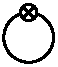
\includegraphics{frg/diagrams/FRG-wetterichEq-FS0_1_1.pdf}\end{gathered}\label{eq:WetterichEq}\,,
\end{align}
where we still use \fs{} notation (instead of a super-trace) for a unified treatment of fermionic (Grassmann-valued) and bosonic (non-Grassmann-valued) fields collected in $\FSsf$ as well as our \rgtime{} derivative with $k=k(t)\equiv \Lambda\eu^{-t}\Rightarrow \partial_t\rightarrow -k\partial_k$.

Recalling \cref{eq:GkabImplicit} we note that the propagator $\FSpropagator{\FSidx{a},\FSidx{b}}[\FSsf]$ on the \rhs{} of the \frgEquation{} depends on the inverse Hessian of $\FSeaa_k[\FSsf]+\Delta S_k[\FSsf]$ and thus on the second functional derivatives of $\FSeaa_k[\FSsf]$.
Therefore the Wetterich equation manifests as a non-linear functional differential equation for the \eaa{}.
The \rhs{} of \cref{eq:WetterichEq} is a non-perturbative one-loop equation since it involves the full scale-dependent propagator $\FSpropagator{\FSidx{a},\FSidx{b}}[\FSsf]$ (solid black line in diagrams) of the theory contracted with the regulator insertion $\FSregulatorDt{\FSidx{b},\FSidx{a}}$ (black cross within a circle in diagrams).
In \cref{eq:WetterichEq} we further introduced the symbolic abbreviation $\FRGflow_k[\FSsf]$\footnote{%
	Note that through the propagator $\FRGflow_k[\FSsf]$ is a non-linear functional of $\FSeaa_k[\FSsf]$ \dash{} its matrix of second functional derivatives/two-point functions to be precise \dash{} and of the regulator, \ie{}, $\FRGflow_k[\FSsf]\equiv\FRGflow_k[\FSeaa_k,R_k;\FSsf]$.
	Symbolic integration of the \frgEquation{} over the \frg{} flux $\FRGflow_k[\FSsf]$ in \rgtime{} is to be understood as solving the functional differential equation in \rgtime{}.%
} for the \textit{\frg{} flux} on the \rhs{}, which will be particularly useful in \cref{subsec:RGconsistency}.
The \frgEquation{} is the governing master equation of the \frg{} framework and it can be used as a generating equation for explicit flow equations for higher-order \nptFunctions{}, see \cref{subsec:higherOrderFlowEquations} for details.

\subsubsection{Regulators, initial condition, and implementation of Wilson's RG approach}\label{subsubsec:regulator}
For the subsequent discussions, regarding the regulator and \ic{} for the Wetterich equation, the following functional integral representation \eqref{eq:EEAint} for the \eaa{} $\FSeaa_k[\FSmf{\FSsf}]$ will be useful.
Using \cref{eq:Gammak} with the definitions \eqref{eq:ZkDef} and \eqref{eq:WkDef} for $Z_k$ and $W_k$ respectively we arrive at
\begin{align}
\stepcounter{equation}\newSubEqBlock
\eu^{-\FSeaa_k[\FSmf{\FSsf}]}
%&=\int\mathcal{D}[\FSff{\FSsf}] \exp\del[3]{-\Sinit[\FSff{\FSsf}]-\Delta S_k[ \FSff{\FSsf}]+\FSmfu{J}{m}\FSffd{\FSsf}{m} +\Delta S_k[ \FSmf{\FSsf}]- \FSmfu{J}{m}\FSmfd{\FSsf}{m} }\\
&= \int \mathcal{D}[\FSff{\FSsf}] \exp\Big(-\Sinit[\FSff{\FSsf}]+\FSmfu{J}{m}\del{\FSffd{\FSsf}{m}-\FSmfd{\FSsf}{m}} 
-\frac{1}{2}\FSregulator{\FSidx{m},\FSidx{n}}\del{\FSffd{\FSsf}{n}\FSffd{\FSsf}{m}-\FSmfd{\FSsf}{n}\FSmfd{\FSsf}{m}}
\Big)\,=\subEqTag \label{eq:EEAintA}\\
%&= \int \mathcal{D}[\FSff{\FSsf}] \exp\del[3]{-\Sinit[\FSmf{\FSsf}+\FSff{\FSsf}]+\FSmfu{J}{m}\FSffd{\FSsf}{m}
%-\frac{1}{2}\FSregulator{\FSidx{m},\FSidx{n}}\del{\del{\FSmfd{\FSsf}{n}+\FSffd{\FSsf}{n}}\del{\FSmfd{\FSsf}{m}+\FSffd{\FSsf}{m}}-\FSmfd{\FSsf}{n}\FSmfd{\FSsf}{m}}
%}\\
&=\int \mathcal{D}[\FSff{\FSsf}] \exp\Big(-\Sinit[\FSmf{\FSsf}+\FSff{\FSsf}]+\FSmfu{J}{m}\FSffd{\FSsf}{m}
-\frac{1}{2}\FSregulator{\FSidx{m},\FSidx{n}}\FSffd{\FSsf}{n}\FSffd{\FSsf}{m} -\FSregulator{\FSidx{m},\FSidx{n}}\FSffd{\FSsf}{n}\FSmfd{\FSsf}{m}
\Big)\,=\subEqTag\label{eq:EEAintB}\\
&=\int \mathcal{D}[\FSff{\FSsf}] \exp\Big(-\Sinit[\FSmf{\FSsf}+\FSff{\FSsf}]+\FSeaa_k^{,\FSidx{m}}[\FSmf{\FSsf}]\FSffd{\FSsf}{m}+\FSffd{\FSsf}{m}\Delta S_k^{,\FSidx{m}}[\FSmf{\FSsf}]\,-\notag\\
&\qquad\qquad\qquad\qquad\qquad\qquad\qquad\qquad-\frac{1}{2}\FSregulator{\FSidx{m},\FSidx{n}}\FSffd{\FSsf}{n}\FSffd{\FSsf}{m} -\FSregulator{\FSidx{m},\FSidx{n}}\FSffd{\FSsf}{n}\FSmfd{\FSsf}{m}
\Big)\subEqTag \label{eq:EEAintC}\\
%&=\int \mathcal{D}[\FSff{\FSsf}] \exp\del[3]{-\Sinit[\FSmf{\FSsf}+\FSff{\FSsf}] - \Delta S_k[\FSff{\FSsf}] +\FSffd{\FSsf}{m}\FSeaa_k^{,\FSidx{m}}[\FSmf{\FSsf}]+\FSffd{\FSsf}{m}\FSregulator{\FSidx{n},\FSidx{m}}\FSmfd{\FSsf}{n}
 %-\FSregulator{\FSidx{m},\FSidx{n}}\FSffd{\FSsf}{n}\FSmfd{\FSsf}{m}
%}\\
\eu^{-\FSeaa_k[\FSmf{\FSsf}]}&=\int \mathcal{D}[\FSff{\FSsf}] \exp\bigg(-\Sinit[\FSmf{\FSsf}+\FSff{\FSsf}] - \Delta S_k[\FSff{\FSsf}] +\frac{\delta\FSeaa_k[\FSmf{\FSsf}]}{\delta \FSmfd{\FSsf}{m}}\FSffd{\FSsf}{m} 
\bigg)\,\label{eq:EEAint}
\end{align}
where we shifted the integration variable according to $\FSff{\FSsf}\rightarrow \FSff{\FSsf} +\FSmf{\FSsf}$ in \cref{eq:EEAintA} and eliminated the source realizing the supremum $\FSmf{J}$ by means of the \qeom{} \eqref{eq:QEOM} in \cref{eq:EEAintC}.\bigskip

In the following we will discuss the necessary properties of the regulator $R_k^{\MFphi\MFphi}(p^2)$,
\begin{align}
R_k^{\FSf{\MFphi}_p,\FSf{\MFphi}_{p'}}=R_k^{\FSf{\MFphi}\FSf{\MFphi}}(p^2)(2\piu)^d\delta^{(d)}(p-p')\equiv p^2 r(p^2/k^2) (2\piu)^d\delta^{(d)}(p-p'),
\end{align}
related to the implementation of Wilson's \rg{} approach for the bosonic FS components in $d$ dimensions, \cf{} \cref{app:fourier} for related conventions.
Regulators related to Grassmann-valued field components inherit similar properties modulo some modifications accounting for internal structure. In the end we will always use a unified regulator scheme for all fields completely specified by a regulator shape function $r(y)$ with the dimensionless ratio 
\begin{align}
	y\equiv \frac{p^2}{k^2},
	\label{eq:yofpkDef}
\end{align}
of the momentum squared to the \rgscale{} squared.

Inserting regulator terms $\Delta S$ in the generating functionals of quantum field theories is not unique to the \frg{}.
Similar or in certain limits even equivalent flow equations to the Wetterich equation in fact preceded it.
Prominent examples are the Wegner-Houghton equation of the seminal paper~\cite{Wegner:1972ih} or the functional variant~\cite{Symanzik:1971cu,Symanzik:1971vw,Alexandre:2000eg} of the well known Callan-Symanzik equation~\cite{Callan:1970yg,Symanzik:1970rt}.
The specific properties of the regulator insertion put forward with the Wetterich equation~\cite{\frgWetterichEq} distinguishes the \frg{} from earlier (functional) \rg{} approaches.
Certain constraints on $R_k$ (or $r(y)$ respectively) are imperative to the correct and explicit implementation of Wilson's non-perturbative continuum \rg{} approach~\cite{Wilson:1971bg,Wilson:1971dh,Wilson:1979qg} outlined in the introduction of this \cref{sec:FRG}.
Only a suitable regulator choice enables sensible computations in the \frg{} approach for a theory at hand.

The four major constraints on $R_k^{\FSf{\MFphi}\FSf{\MFphi}}(p^2)$ are:
\begin{enumerate}
	\item \phantomsection\label{paragraph:regulatorIR}\textbf{Infrared finiteness:}
	\begin{align}
	\lim_{p^2/k^2\rightarrow 0 }R_k^{\FSf{\MFphi}\FSf{\MFphi}}(p^2)>0 \qquad (\text{typically }\sim k^2).\label{eq:RkBIR}
	\end{align}
	The quadratic ansatz \eqref{eq:DeltaSRab} together with the requirement of \cref{eq:RkBIR} introduces a mass term (typically $\sim k^2$) for the low momentum modes, $p^2<k^2$, of $\FSf{\MFphi}$. This additional mass term suppresses fluctuations of those low momentum components in the functional integral \eqref{eq:ZkDef} and regularizes the theory in the \ir{}.
	
	\item \phantomsection\label{paragraph:regulatorHighP}\textbf{Vanishing for high momentum modes:} For fields with momenta larger than the current scale, $p^2>k^2$ the regulator has to vanish in the limit
	\begin{align}
	\lim_{p^2/k^2\rightarrow \infty }R_k^{\FSf{\MFphi}\FSf{\MFphi}}(p^2)=0 \label{eq:RkBUV}
	\end{align}
	in $d$ dimensions at least with $(p^2)^{(d-1)/2}R_k(p^2)\rightarrow 0$~\cite{Pawlowski:2015mlf,PawlowskiScript}. 
	This property implies for $k\rightarrow 0$ \dash{} in the physical limit \dash{} that all regulator-dependencies drop out and all generating functionals ($Z_k$, $W_k$ and $\FSeaa_k$) include the full effect of all quantum fluctuations.
	In other words, the introduction of a suitable regulator does not spoil the physical \ir{} observables extracted from these generating functionals at $k\rightarrow 0$.
	The requirement of \cref{eq:RkBUV} implies in the \uv{}, $p^2/k^2\gg 1$, the vanishing of the \rgscale{} derivative $\partial_k R_k^{\FSf{\MFphi}\FSf{\MFphi}}(p^2)$, which ensures \uv{} finiteness.
	Regulators fulfilling \cref{eq:RkBIR,eq:RkBUV} typically have a \rg{}-scale derivative $\partial_k R_k^{\FSf{\MFphi}\FSf{\MFphi}}(p^2)$ which peaks around the momentum shell $p\sim k$ and thus the contributions from fields with momenta $\sim k$ dominate in the functional integral. This notion of momentum locality of \rg{} steps implements Wilson's non-perturbative \rg{} approach~\cite{Wilson:1971bg,Wilson:1971dh,Wilson:1979qg} of integrating out fluctuations momentum shell by momentum shell. 
	
	\item \phantomsection\label{paragraph:regulatorUV}\textbf{Diverging in the ultraviolet:} For $k\rightarrow \Lambda$, where $\Lambda$ is an \uv{} initial scale which should be larger than all relevant physical scales of the problem at hand, the regulator should diverge
	\begin{align}
	\lim_{k\rightarrow \Lambda} R_k^{\FSf{\MFphi}\FSf{\MFphi}}(p^2)=\infty.
	\end{align}
	This can be discussed explicitly for the \eaa{} $\FSeaa_k$ using its integral representation \eqref{eq:EEAint}: the regulator insertion $\Delta S_k[\FSff{\FSsf}]$ in \eqref{eq:ZkDef} diverges for $k\rightarrow \Lambda$ and thus dominates the functional integral on the \rhs{}
	In this limit $\Delta S_k[\FSff{\FSsf}]$ acts as a functional delta distribution~\cite{Wetterich:2001kra,Gies:2006wv} and the functional integral on the \rhs{} of \cref{eq:EEAint} can be evaluated to $\exp(-\Sinit[\FSmf{\FSsf}])$.
	Subsequently the \rgscaledependent{} \eaa{} $\FSeaa_\Lambda[\FSmf{\FSsf}]$ at the \uv{} initial scale $\Lambda$ reduces to the classical action $\Sinit[\FSmf{\FSsf}]$.
	
	Depending on the theory at hand, the explicit choice of regulator (shape function), and the chosen \uv{} initial scale $\Lambda$, the simple identification of a plain classical action $S[\FSmf{\FSsf}]$ as \ic{} at $k=\Lambda$ for $\FSeaa_k[\FSmf{\FSsf}]$ might be insufficient especially when working with a finite \uv{} initial scale $\Lambda$.
	Subtleties related to the chosen normalization of generating functionals, renormalization procedure, and potentially gauge fixing might require the addition of suitable (counter) terms at $k=\Lambda$ and thus a modified \ic{} $S_\Lambda[\FSmf{\FSsf}]$, see, \eg{}, \ccite{Pawlowski:2005xe,PawlowskiScript,Braun:2018svj}. 
	The concept of renormalization group consistency discussed in \cref{subsec:RGconsistency} is closely related to the proper choice of $S_\Lambda[\FSmf{\FSsf}]$.
	We will discuss problem/theory specific subtleties further when we introduce the \ics{} for the explicit \frg{} flows considered within this work.
	See, \eg{}, \cref{paragraph:ONRGconsistency}, \cref{subsec:UUV}, and \cref{sec:cdwmf}.
	
	\item \phantomsection\label{paragraph:regulatorSym}\textbf{Symmetry considerations:} The regulator should not break any symmetries of the theory, \ie{}, its functional integral.
	Prime examples of such symmetries are chiral or $O(N)$ symmetries and for the relativistic theories considered here \Poincare{} invariance.
	If a regulator choice breaks such a symmetry computed observables might be spoiled by this artificial, explicit symmetry breaking.
	This situation might be remedied by introducing appropriate counter terms in $S_\Lambda[\FSmf{\FSsf}]$, \cf{} \cref{subsec:renomMF}, or in case of the breaking of gauge symmetry by a more elaborate construction, \cf{} \cref{paragraph:qcdGF}.
\end{enumerate}

The first three constraints related to the finiteness \dash{} proper regularization and \ic{} for the \frg{} flow \dash{} in practice often compete with symmetry considerations like \Poincare{} invariance and related causality issues (unphysical poles in the complex frequency plane) arising during analytical continuation to real time quantities, for details, see, \eg{}, Sec. II of \ccite{Braun:2022mgx} and references therein.
Furthermore, computational and numerical practicability considerations can conflict with especially symmetry considerations.
A prime example of the latter is the use of purely spatial regulators in our computations of \cref{chap:GN,chap:QMM} which introduces an explicit breaking of \Poincare{} invariance. 
The use of purely spatial regulators is mainly motivated by the facilitation or at least significant simplification of computations at non-zero temperature.

An explicit choice of regulator (shape function) is usually made weighing the different constraints and practicability/feasibility considerations.
Common and in some cases even established regulator choices often strongly vary depending on the problem at hand, the employed truncation, \cf{} \cref{subsubsec:truncation}, and scope of the investigation.
Further details on the vast and important topic of adequate regulator choice in the \frg{} framework can be found in \ccite{Litim:2000ci,Litim:2001up,Pawlowski:2005xe,Rosten:2010vm,Osborn:2011kw,Pawlowski:2015mlf,Braun:2017srn,Braun:2020bhy,DePolsi:2022wyb,Otto:2022jzl,Braun:2022mgx,Ihssen:2023xlp,Zorbach:2024zjx} and references therein.

\fullWidthFigure%
	{frg/figures/regulator_shape_functions.pdf}% Graphics
	[fig:rShape_plain,fig:rShape_derivative]% Sublabels
	{%
		Plots of selected \dash{} \cf{} \cref{eq:rflat,eq:rsharp,eq:rlambdaDef} \dash{} regulator shape functions on the left \subref{fig:rShape_plain} and their derivatives on the right \subref{fig:rShape_derivative}.
		In terms of its properties the exponential regulator (shape function) $r_\mathrm{exp}(y)$ may be considered as an archetypical \frg{} regulator implementing Wilson's \rg{} approach with a smooth focusing around $p=k$ and many sketches of \frg{} regulators, see, \eg{}, Fig. 1 of \ccite{Gies:2006wv}, resemble its plot here.%
	}%Caption
	{fig:rShape}%Label
In this work we will employ regulators related to three explicit regulator shape functions (presented in the notation of Table 1 of \ccite{Pawlowski:2015mlf}): the flat (\acrshort{lpa} optimized Litim) regulator~\nbcite{Litim:2000ci,Litim:2001up}
\begin{align}
	r_\mathrm{flat}(y)\equiv\del{\frac{1}{y}-1}\mkern-1.5mu\thetaLitim(1-y)\,,
\label{eq:rflat}
\end{align}
the step-like sharp regulator
\begin{align}
	r_\mathrm{sharp}(y)\equiv\frac{c}{y}\mkern1.5mu\thetaLitim(1-y)\,,
\label{eq:rsharp}
\end{align}
in the limit $c\rightarrow\infty$, and the exponential regulator
\begin{align}
	r_\mathrm{exp}(y)\equiv\del{\exp(y)-1}^{-1}\,.
\label{eq:rexp}
\end{align}
When working with these shape functions it is convenient to define 
\begin{align}
	\lambda(y)\equiv r(y)+1
	\label{eq:rlambdaDef}
\end{align}
as well as fermionic $\rf(y)$ and bosonic $\rb(y)$ shape functions related by
\begin{align}
	\lambda(y)\equiv r(y)+1\equiv \rb(y)+1\equiv(\rf(y)+1)^2\, .
	\label{eq:rfrbDef}
\end{align}
The three shape functions and their derivatives are visualized in \cref{fig:rShape}.
The particular choice of how the shape functions \eqref{eq:rflat}--\eqref{eq:rexp} and their derivatives are plotted in \cref{fig:rShape} is based on their appearance in explicit expressions, \cf{} \cref{eq:cdwFlow,eq:cdwFlow}.
This visualization complements the discussion of finiteness and the related first three constraints on $R_k^{\FSf{\MFphi}\FSf{\MFphi}}(p^2)$ which can be directly translated to constraints\footnote{%
	The constraints \cref{eq:ryA,eq:ryC} \dash{} \textit{infrared finiteness} and \textit{diverging in the ultraviolet} \dash{} are on the level of the regulator shape function $r(y)$ closely linked.
	Indeed considering ${\lim_{y\rightarrow 0 } y\, r(y)=1}$ entails $r(y)\rightarrow1/y$ and thus guarantees \cref{eq:ryC} in the limit $y\rightarrow0$.
} for the shape functions, \cf{} \ccite{Pawlowski:2015mlf},
\begin{subequations}\label{eq:ry}
\begin{align}
	\lim_{y\rightarrow 0 } y\, r(y)&>0\qquad (\text{typically }1)\,,\label{eq:ryA}\\
	\lim_{y\rightarrow \infty,\,\epsilon>0 } y^{\frac{d}{2}+\epsilon}r(y)&=0\,,\label{eq:ryB}\\
	\lim_{y\rightarrow 0 } r(y)&=\infty\,.\label{eq:ryC}
\end{align}
\end{subequations}
The flat regulator shape function is optimized~\cite{Litim:2000ci,Litim:2001up} for \acrshort{lpa} computations, \cf{} \cref{subsubsec:truncation}, in the sense that this regulator choice maximizes the gap in the inverse propagator which according to \ccite{Litim:2000ci} provides the greatest stability of the flow.
For additional details and a refined view of regulator optimization with a strong \cfd{} perspective we refer the interested reader to \ccite{Zorbach:2024zjx}.
Additionally the step function in \cref{eq:rflat} usually allows for a symbolic evaluation of momentum integrals and thus much simpler flow equations.
We will employ the flat and the sharp regulator shape functions in \cref{chap:GN}.
The latter is particularly useful in \mf{} computations since it also allows for a symbolic evaluation of momentum integrals and one usually recovers expressions known from conventional \mf{} computations with a sharp cutoff, \cf{} \cref{sec:gnInfInhomo} and, \eg{}, \ccite{Braun:2018svj}.
The exponential regulator shape function $r_\mathrm{exp}(y)$ is smooth and thus has certain advantages in explicit numerical computations, which we will leverage in \cref{chap:QMM}.

\subsubsection{Truncation and projection strategies}\label{subsubsec:truncation}
With a suitable regulator choice according to the previous \cref{subsubsec:regulator} the Wetterich equation is exact, hence the synonym \erg{} for \frg{}.
By construction the \ir{} physics, \ie{}, physical observables, are independent from the specific regulator choice as long as the regulator adheres to the previously established constraints.
Exact in this context means solving the evolution equations \eqref{eq:WetterichGeneral} or \eqref{eq:WetterichEq} with a suitable \ic{} and regulator choice from the \uv{} down to the \ir{} amounts to solving the underlying functional integral without any approximations.
The blue lines in \cref{fig:truncation} represent two exact \rg{} trajectories with different suitable regulators.
Using the full/untruncated Wetterich equation, the \ir{} physics encoded in $\FSeaa_0[\FSsf]$ is indeed regulator independent.
The \rg{} trajectories through theory space differ however for distinct regulators.
Flowing from $\FSeaa_\Lambda[\FSsf]$ to $\FSeaa_0[\FSsf]$, one gains access to the full quantum effective action $\FSeaa_0[\FSsf]=\Gamma_\mathrm{1PI}[\FSsf]$ and all related physical observables of the macroscopic theory prescribed by the microscopic action under consideration.

The issue a \frg{} practitioner faces however is one of \textit{conservation of complexity}: solving the underlying functional integral for strongly interacting theories is at best an extremely involved task and often practically impossible.
The functional flow equation for $\FSeaa_k[\FSsf]$ elegantly eliminates the need for the computation of the complicated functional integral at the cost of introducing a complicated functional differential equation to be solved.
Solving such equations without truncations or simplifying approximations is usually not possible for interacting \qfts{}, as there are no explicit numeric or symbolic methods to solve the arising non-linear functional differential equations.
One notable exception are applications of the \frg{} to models in zero dimensions, which will be discussed at length in \cref{chap:zeroONSU2}.
For theories in non-zero dimensions truncation schemes for the Wetterich equation are required to project from the full/exact functional differential equation onto a finite set of \pdes{} or even \odes{}.
For such differential equations numeric and in some cases even symbolic/analytic solution methods exist, which both facilitate practical computations in the \frg{} framework.
However with a truncation to a finite set of non-functional differential equations the \frg{} is no longer exact due to the simplifying steps taken and furthermore results computed in a truncation may explicitly depend on the specific regulator choice even for completely valid regulators.
This situation is visualized in \cref{fig:truncation} together with the untruncated/exact solution.
The red and green curves in \cref{fig:truncation} represent the flow using two different truncations: the regulator-dependence and derivation from the exact result for $\FSeaa_0[\FSsf]$ are clearly visualized in the \ir{} at $k=0$.
The truncation $t_2$ in \cref{fig:truncation} in green represent a systematic improvement over the truncation $t_1$ in red denoted by a weaker regulator-dependence and better error in the \ir{}.
Specifying errors related to truncation and regulator choice in the \frg{} can be extremely involved, especially when studying strongly interacting theories.
The process usually involves improving the truncation in a systematic way and comparing results obtained at varying levels of improvement to check for an apparent convergence of the chosen truncation and improvement scheme.

In the following we will briefly discuss four common truncation schemes. For details we refer to literature~\cite{Berges:2000ew,PawlowskiScript,Gies:2006wv,Kopietz:2010zz,Wetterich:2001kra,Pawlowski:2005xe,Rosten:2010vm,Delamotte:2007pf,Dupuis:2020fhh} and our applications in \cref{chap:zeroONSU2,chap:GN,chap:QMM}.
\fullWidthFigure%
	{frg/figures/truncation.pdf}% Graphics
	[]% Sublabels
	{Schematic \frg{} flow \dash{} \rgscaleevolution{} of the \eaa{} in the space of its couplings $\{\lambda_i\}$ for different regulators $R_1$ and $R_2$ (solid and dashed lines) and assuming an exact solution of the full Wetterich equation (blue lines) or solutions of the truncated Wetterich equation using two truncations $t_1$ and $t_2$ (red and green lines). Truncation $t_2$ is considered to be a systematic improvement of truncation $t_1$. }%Caption
	{fig:truncation}%Label

\paragraph{Vertex expansion}\phantomsection\label{paragraph:vertexExpansion}\mbox{} \\
Arguably the most natural truncation and expansion scheme for the \frgEquation{} is the so-called \textit{vertex expansion}.
The idea is to expand the \rgscaledependent{} \eaa{} $\FSeaa_k[\FSmf{\FSsf}]$ in its moments \dash{} in correlation functions \dash{} $\FSeaa_k^{(n)}(\FSmf{\FSsf}_0)$ around the expansion point $\FSmf{\FSsf}_0$ with
\begin{align}
\FSeaa_k[\FSmf{\FSsf}]\equiv\lim_{N\rightarrow\infty}\FSeaa_k^N[\FSmf{\FSsf}]\equiv\lim_{N\rightarrow\infty}\sum_{\{n\}=\{0\}}^{\{N\}} \FSeaa_k^{(n)}(\FSmf{\FSsf}_0)\prod_{i\in \{n\}}(\FSmf{\FSsf}_i-\FSmf{\FSsf}_{0,i})\,,\label{eq:vertexAnsatz}
\end{align}
where integration and summation over internal indices (position, flavor,$\ldots$) is implied and all \ipi{} vertices of theory are summed up in $\FSeaa_k^N[\FSmf{\FSsf}]$ up to order $N$.
Inserting the ansatz \eqref{eq:vertexAnsatz} into the \frgEquation{} one can use functional derivatives in the spirit of \cref{subsec:higherOrderFlowEquations} to generate an infinite tower of coupled \odes{} for all \ipi{} vertices
\begin{subequations}\label{eq:vertexTower}
\begin{align}
	\partial_t\FSeaa_k^{\{0\}}(\FSmf{\FSsf}_0)=&\,\FRGflow_k^{\{0\}}\mkern-3mu\del{\mkern2mu\FSeaa_k^{\{2\}};\FSmf{\FSsf}_0}\,,\\
	\partial_t\FSeaa_k^{\{1\}}(\FSmf{\FSsf}_0)=&\,\FRGflow_k^{\{1\}}\mkern-3mu\del{\mkern2mu\FSeaa_k^{\{2\}},\FSeaa_k^{\{3\}};\FSmf{\FSsf}_0}\,,\\
	\partial_t\FSeaa_k^{\{2\}}(\FSmf{\FSsf}_0)=&\,\FRGflow_k^{\{2\}}\mkern-3mu\del{\mkern2mu\FSeaa_k^{\{2\}},\FSeaa_k^{\{3\}},\FSeaa_k^{\{4\}};\FSmf{\FSsf}_0}\,,\\* % prohibits a page break here
	\vdots\mkern5mu&\notag
\end{align}
\end{subequations}
The \rhs{} of the flow equation for a \ipi{} vertex of order $n$ contains only the propagator $G_k$ (which non-linearly depends on the two-point functions), \ipi{} vertices up to order $n+2$, and the regulator insertion while maintaining one-loop structure.
We may also note that the zero-point function $\FSeaa_k^{(0)}(\FSmf{\FSsf}_0)$ does not couple back into the system.

One may expect good convergence of the tower of equations \eqref{eq:vertexTower}, if the higher-order \nptFunctions{} are suppressed.
Such a suppression motivates a truncation of the infinite tower up to order $N$ considering only $\FSeaa_k[\FSmf{\FSsf}]=\FSeaa_k^N[\FSmf{\FSsf}]$.
The infinite tower gets truncated up to order $N$ by either neglecting the flow of $\FSeaa_k^{\{N+1\}}(\FSmf{\FSsf}_0)$ and $\FSeaa_k^{\{N+2\}}(\FSmf{\FSsf}_0)$ or approximating the vertices, for the latter approach, see, \eg{}, \ccite{Blaizot:2005xy}.
When properly tracking the momentum dependence of the involved \ipi{} vertices, \cf{} the works~\cite{Blaizot:2004qa,Blaizot:2006vr, Blaizot:2006ak} of Jean-Paul Blaizot \etal{} and \ccite{Ledowski:2004zz,Sinner:2007ws,Kopietz:2010zz} of Peter Kopietz \etal{}, this approach provides excellent resolution in momentum space while having limited resolution in field space due to the expansion of the \eaa{} in \ipi{} vertices.
Due to the rapidly growing complexity of the flow equations when increasing $N$, practical computations are typically limited to a rather small order between $N=4$ and $N=6$.
The high resolution in momentum space and proper resolution of the momentum-dependence of the involved \ipi{} vertices makes the vertex expansion a very attractive expansion scheme for quantum many-particle systems in condensed matter physics, see, \eg{}, \ccite{Ledowski2004Jun,Benitez:2009xg,Boettcher:2012cm,Metzner2012Mar}, \hep{} and especially for Yang-Mills theories and \qcd{}, see, \eg{}, \ccite{Reuter:1993kw,Wetterich:1996kf,Gies:2002af,Braun:2014ata,Cyrol:2017ewj,Alkofer:2018guy,Fu:2019hdw}, and quantum gravity, see, \eg{}, \ccite{Reuter:1996cp,Christiansen:2015rva,Meibohm:2015twa,Eichhorn:2018akn,FuQCDRev}.
An overview and further relevant literature may be found in the Secs. 4, 5, and 6 of review~\cite{Dupuis:2020fhh}.
When studying symmetry breaking \dash{}  especially around phase transitions \dash{} the vertex expansion is of limited use since studies of such phenomena require a higher resolution in field space. 
Both symmetry breaking and also bound states can enhance higher-order \nptFunctions{} limiting or even destabilizing the vertex expansion, see also the discussion in the following paragraph \customref{paragraph:taylorExpansion}{Taylor and other global expansions}.
In this work we are mainly interested in the study of strongly coupled theories in field space and symmetry breaking in those systems. 
Thus we do not use the vertex expansion beyond the benchmark study of \cref{subsubsec:vertex_expansion,paragraph:sc2taylorFlow} in zero dimensions.

\paragraph{Derivative expansion and the local potential approximation}\phantomsection\label{paragraph:derivativeExpansion}\mbox{} \\
The main \frg{} expansion scheme employed in this work is the \de{}, which is a well established expansion and truncation scheme for the Wetterich equation in applications that require high resolution in field space, see, \eg{}, the review~\cite{Dupuis:2020fhh} and references therein.
Prime examples are the zero-dimensional theories we study in \cref{chap:zeroONSU2} and the \loefts{} we discuss in \cref{chap:GN,chap:QMM}.
The underlying idea behind the \de{} is to expand the \rgscaledependent{} \eaa{} $\FSeaa_k[\FSmf{\FSsf}]$ in powers of momenta \dash{} \ie{}, derivatives in position space, hence the name \de{}.
Such an expansion is justified when studying long range physics at small momentum scales $p^2$ satisfying
\begin{align}
	\frac{p^2}{s_k^2}\ll 1\,,
	\label{eq:deMomenta}
\end{align}
where $s_k$ is a theory specific \ir{} mass/momentum scale.
Even in theories without a physical mass gap $m_\gap$ the regulators used in the \frg{} provide an \ir{} regularization at finite $k$ and the characteristic scale $s_k$ is typically
\begin{align}
	s_k^2\approx m_\gap^2+k^2\,.
	\label{eq:dexikDef}
\end{align}
Considering the regulator properties discussed in \cref{subsubsec:regulator} we may indeed note that the regulator insertion $\partial_t R_k$ in the \frgEquation{} suppresses momenta $p^2\smallergtrsim k^2$ by focusing the integration over internal loop momenta around $p=k$, which is visualized in \cref{fig:rShape_derivative}.
The aforementioned suppression of high momentum modes renders the condition $p^2/k^2\smallerlesssim 1$ valid in the loop of the Wetterich equation.
This in turn implies that the condition~\eqref{eq:deMomenta} is indeed fulfilled \dash{} even for theories without a physical \ir{} mass gap $m_\gap$, \cf{} \cref{eq:dexikDef}.
A proper, \ie{}, for a given truncation optimized, regulator can greatly improve the stability and apparent convergence of the \de{}~\cite{Pawlowski:2005xe,Litim:2000ci,Litim:2001up}.
For the lowest-order \de{} \dash{} the so-called \acrrepeat{lpa}, which we will introduce in the following \dash{} the flat regulator that we introduced via its shape function in \cref{eq:rflat} is such an optimized regulator.

To illustrate the \de{} and related truncation strategies let us consider a theory of $N$ interacting scalar fields $\vec{\phi}$ with \ON{} symmetry in $d$ dimensions and corresponding mean-fields $\vec{\varphi}$ .
To lowest, zeroth-order \de{} \dash{} \ie{}, in \lpa{} \dash{} the \rgscaledependent{} \eaa{} is simply given by
\begin{align}
	\FSeaa_k^{\mathrm{DE}_0}\sbr{\vec{\varphi}\mkern2mu}\equiv\FSeaa_k^\mathrm{LPA}\sbr{\vec{\varphi}\mkern2mu}\equiv\int_x\del[3]{\frac{1}{2}\partial_\mu\varphi_i\partial_\mu\varphi_i+\Ukrho{}}\,,
	\label{eq:deLPA}
\end{align}
with $\varrho\equiv\varphi_i\varphi_i/2$ and the \rgscaledependent{}, \ON{}-symmetric self-interaction potential $\Ukrho{}$ as the only scale-dependent quantity.
Quantum fluctuations at $\order(\partial^2)$ and above are neglected and only the classical kinetic \dash{} without a running wave-function renormalization \dash{} is included~\cite{Reuter:1993rm,Morris:1994ki}.

The \rgscaledependent{} local potential can be evolved from the \uv{} at $k=\Lambda$ to the \ir{} $k\rightarrow 0$ using the \frgEq{}.
In the \ir{} $U_{k=0}\del{\varrho}$ can be identified with (contributes to) the effective potential $\VeffFArgs{\muT;\FSsf}$, see \cref{app:grandCanonicalPartitionFunction} and \cref{eq:VeffFdef}, when considering homogeneous (inhomogeneous) condensates. 
Thus $\Ukrho{}$ and especially $U_{k=0}\del{\varrho}$ play a critical role in the study of symmetry breaking and thermodynamics.
Further more the \lpa{} can be used for mean-field and large-$N$ computations, see, \eg{}, \cref{subsec:0dONresults,sec:gnInfInhomo,sec:gnInfHomo,sec:cdwmf}. 

The explicit flow equations for the local potential $\partial_t \Ukrho{}$ manifest in practice as \pdes{}, see, \eg{}, \cref{eq:pde_gamma,eq:flow_equation_effective_potential,eq:SU2model0dUFlow,eq:pdeq-U,eq:cdwFlow} in the main parts~\ref{chap:zeroONSU2}, \ref{chap:GN}, and \ref{chap:QMM} of this work.
As alluded to in the introduction~\ref{chap:introduction}, various collocation methods, \cf{} \ccite{\frgFDReferences,\frgSplineReferences} and also expansion schemes discussed in the \customref{paragraph:taylorExpansion}{next paragraph} are common and established in the \frg{} community to solve \lpa{} flow equations \dash{} the explicit \pdes{} for $\Ukrho{}$.
The \fd{} and spline collocation methods used, are however based on the often tacit assumption, that $\Ukrho{}$ is smooth.
This is however, as we argue at length in \cref{chap:zeroONSU2} and demonstrate also in \cref{chap:GN}, \apriori{} and also in prominent scenarios \aposteriori{}, in general not a valid assumption.
It has been established within the last few years by us and collaborators, \cf{} Refs.~\cite{Grossi:2019urj,zerod1,zerod2,zerod3,Ihssen2020,Grossi:2021ksl,Stoll:2021ori,Ihssen:2022xkr,Ihssen:2023xlp} and \cref{subsec:RGflow} as well as \cref{chap:zeroONSU2,chap:GN}, that the \frg{} flow equations \dash{} the \lpa{} flow equation as a truncated one, most prominently included \dash{} are non-linear conservation/convection equations.
Their non-linearity as well as explicit source/sink terms, \cf{} \cref{paragraph:chemical_potential_shock_wave}, can lead to discontinuities in $\partial_\MFrho \Ukrho{}$ and thus kinks in $\Ukrho{}$ which explains the poor (numerical) performance of the established ``grid methods''.
The adaptation of more suited numerical methods from the field of \cfd{}, see \cref{sec:conservationLaws}, is one major part of our research~\cite{zerod1,zerod2,zerod3,zerod4,Stoll:2021ori} discussed in \cref{chap:zeroONSU2,chap:GN}.\bigskip

The first systematic improvement $\mathrm{DE}_2$ in the \de{} to \lpa{}
\begin{align}
	\FSeaa_k^{\mathrm{DE}_2}\sbr{\vec{\varphi}\mkern2mu}=\int_x\del[3]{\frac{1}{2}Z_k(\varrho)\partial_\mu\varphi_i\partial_\mu\varphi_i+\frac{1}{4}Y_k(\varrho)\partial_\mu\varrho\partial_\mu\varrho+\Ukrho{}}\,,
	\label{eq:deDE2}
\end{align}
includes $\order(\partial^2)$ corrections in form of a field-dependent, running wave-function renormalization $Z_k(\varrho)$ and for $N>1$ an additional term $Y_k(\varrho)\partial_\mu\varrho\partial_\mu\varrho$ due to the difference in transverse and longitudinal fluctuations of $\vec{\varphi}$~\cite{Dupuis:2020fhh,Eser:2019pvd}. 
A very common simplification to $\mathrm{DE}_2$ is called \lpap{} which entails omitting the $Y_k(\varrho)$ contribution and considering only a field-independent $Z_k$.
Given an ansatz for the \eaa{} in \de{} one can proceed to compute the propagators in the given truncation.
The propagators and the ansatz for the \eaa{} can then be inserted into the \frgEquation{} and/or corresponding flow equations for higher-order \nptFunctions{} to project out flow equations for the running couplings.
Those flow equations manifest as \pdes{} or \odes{} allowing for a numerical solution of the Wetterich equation. 
Further details will be discussed in this thesis in \cref{chap:zeroONSU2,chap:GN,chap:QMM} while additional details and references can be found in, \eg{}, Sec. 2.3 of the review~\cite{Dupuis:2020fhh}.

\paragraph{\frg{} Taylor and other global expansions}\phantomsection\label{paragraph:taylorExpansion}\mbox{} \\
The so-called \textit{\frg{} Taylor expansion}, see, \eg{}, \ccite{\frgTaylorReferences}, is closely related to the \customref{paragraph:vertexExpansion}{vertex expansion} and the \lpa{} of the \customref{paragraph:derivativeExpansion}{derivative expansion}.
In the context of the \lpa{} the \frg{} Taylor expansion is simply the expansion of the \rgscaledependent{} local potential in a Taylor series
\begin{align}
	\Ukrho{}=\sum_{n=0}^{N_\nu} \frac{\lambda_{n,k}}{n!}\del{\MFrho-\kappa_k}^n\, ,\label{eq:ukrhoTaylor}
\end{align}
around a potentially scale-depended expansion point $\kappa_k$, with scale-depended moments $\lambda_{n,k}$ and an expansion order $N_\nu$, where we adopt the notation of \ccite{Fu:2022gou}.
Inserting the ansatz \nolinebreak[3]\eqref{eq:ukrhoTaylor} into the \lpa{} flow equation one can project onto the moments $\lambda_{n,k}$ and the expansion point $\kappa_k$ by taking derivatives \wrt{} $\MFrho.$
The \frg{} Taylor expansion includes the zeroth-order contributions in momentum space to the vertex expansion.
As such both \frg{} Taylor and vertex expansion are completely equivalent in zero-dimensional space-time, \cf{} \cref{subsubsec:vertex_expansion,paragraph:sc2taylorFlow}.

With a well chosen, potentially scale depended expansion point and sometimes a rather low number of expansion coefficients, the \frg{} Taylor expansion is an established method within the \frg{} community, see, \eg{}, the certainly incomplete list of \ccite{\frgTaylorReferences}.
However it is also acknowledged, that such a local expansion is rather limited in scenarios where global information about the potential is required, see, \eg{}, \ccite{Fu:2022gou,Pawlowski:2014zaa,PawlowskiScript}.
The study of symmetry breaking and phase transitions, especially first-order phase transitions, is one notable example.
It should however be noted, that an expansion like \cref{eq:ukrhoTaylor} and the projection onto its scale-dependent moments $\lambda_{n,k}$ and expansion point $\kappa_k$, \apriori{} assumes analyticity of $\Ukrho{}$ around the expansion point $\kappa_k$.
This is an incredibly restrictive and assumption that is just not justified for certain applications. 
We will discuss this limitation further in \cref{subsubsec:vertex_expansion,paragraph:sc2taylorFlow} in the context of our studies in zero dimensions.\bigskip

The local nature of the \frg{} Taylor expansion \eqref{eq:ukrhoTaylor} has, to an extent, motivated the adaptation of global pseudo-spectral collocation methods in the \frg{} community for an expansion of $\Ukrho{}$ in Chebyshev polynomials, see, \eg{}, \ccite{\frgChebyshevReferences}.
While this certainly improves upon the \frg{} Taylor expansion by considering a global expansion of the potential $\Ukrho{}$, such collocation methods are still severely limited when non-analyticities come into play.
The application of plain global pseudo-spectral collocation methods to non-linear convection equations including complicated source terms \dash{} like the \lpa{} flow equation \dash{} should be seriously reconsidered.
This is not the personal opinion of my collaborators and me, but rather firmly established knowledge in the field of such pseudo-spectral collocation methods.
It is interesting to note, that most of the aforementioned \frg{} Chebyshev literature references the excellent book \textit{``Chebyshev and Fourier Spectral Methods''}~\cite{boyd2001chebyshev} of John P. Boyd, which in no uncertain terms addresses the clear limitations of global-collocation methods when it comes to non-analyticities and shocks.
The praised exponential and geometric convergence of global-collocation methods is lost in presence of shocks, corner singularities, or discontinuities~\cite{boyd2001chebyshev}.
Spectral filtering, sequence acceleration, spectral reconstruction, or outright discontinuous Galerkin methods (employing pseudo-spectral methods in control volumes, allowing for discontinuities) are mentioned as necessary improvements when applying pseudo-spectral collocation methods to problems involving non-analyticities~\cite{boyd2001chebyshev}.
In plain pseudo-spectral collocation methods such non-analyticities manifest in the frequency spectrum as Wilbraham-Gibbs-type oscillations \nolinebreak[3]\cite{Wilbraham:1848,Gibbs:1898,Gibbs:1899} which without the aforementioned improvements completely destabilize the \ode{} system for the flow of the expansion coefficients.

\paragraph{Perturbative loop expansion}\phantomsection\label{paragraph:loopExpansion}\mbox{} \\
We will conclude the discussion on truncation strategies for the Wetterich equation with a short remark on the \textit{perturbative loop expansion} following \ccite{Papenbrock:1994kf,Litim:2002xm,Braun:2021retreat,PawlowskiScript,Gies:2006wv}.
Conventional renormalized perturbation theory, see, \eg{}, \ccite{Iliopoulos:1974ur,Peskin:1995ev,ZinnJustin:2002ru}, in form of a loop expansion in terms of classical, tree-level propagators can be recovered from the \frg{} in an iterative procedure. 
The $(N+1)$-loop correction to the \ea{} can be computed with the \frgEquation{} by inserting the $N$-loop expression for the propagator $G_k$ into the \rhs{} of \cref{eq:WetterichEq} and integrating the resulting equation from the \uv{} $k=\Lambda$ to the \ir{} $k=0$.

For the sake of simplicity we will consider a quantum field theory of a single scalar field $\phi$ with the classical action $S$ and corresponding mean-field $\varphi$ in the following.
Starting the iterative procedure with the zeroth-order tree-level propagator $G_k=(S^{(2)}+R_k)^{-1}$ and integrating over the \rgscale{}, one obtains the \ea{} to one-loop order
\begin{align}
	\Gamma_{1-\mathrm{loop}}[\varphi]=S[\varphi]+\FSeaa_{\Lambda,1}[\varphi]+\frac{1}{2}\Tr\ln S^{(2)}[\varphi]-\frac{1}{2}\Tr\ln \del[2]{S^{(2)}[\varphi]+R_\Lambda}\, ,
	\label{eq:ea1loop}
\end{align}
with the classical action $S[\varphi]$, a \rg{}-scheme-/regulator-dependent one-loop counter term $\FSeaa_{\Lambda,1}[\varphi]$, the potentially divergent one-loop diagram $\frac{1}{2}\Tr\ln S^{(2)}[\varphi]$, and the \rg{}-scheme-/regulator-dependent diagram $\frac{1}{2}\Tr\ln \del[1]{S^{(2)}[\varphi]+R_\Lambda}$ to cancel the potential divergences in the aforementioned diagram.
Thus the difference $\frac{1}{2}\Tr\ln S^{(2)}[\varphi]-\frac{1}{2}\Tr\ln \del[1]{S^{(2)}[\varphi]+R_\Lambda}$ can be considered as a regularized, finite loop diagram.
The counter term $\FSeaa_{\Lambda,1}[\varphi]$ can be determined by enforcing renormalization group consistency, see \cref{subsec:RGconsistency} for details, which in this context simply entails the independence of the \ea{} $\Gamma[\varphi]$ in the \ir{} of $\Lambda$.
The sum of the classical action and the counter term form the modified \ic{}: $\Sinit[\varphi]=S[\varphi]+\FSeaa_{\Lambda,1}[\varphi]$.

The two-loop result can be obtained by computing the propagator from the one-loop result~\eqref{eq:ea1loop}, inserting the result in the \rhs{} of the \frgEquation{} and again integrating over the \rgscale{}, see, \eg{}, \ccite{Litim:2002xm}.

Using the Wetterich equation as a master equation with the outlined iteration procedure is a simple and robust way to compute expressions for regularized and renormalized \ipi{} correlation functions to any desired perturbative loop-order.
The generation and complete resummation of the perturbative loop expansion also serves as further proof \dash{} beyond the validity and exactness of its derivation \dash{} that the \frgEquation{} is indeed exact.
A perturbative approach/loop expansion has only very limited applicability in the context of our work, since we are interested in strongly interacting systems which are notoriously elusive to tackle with such perturbative techniques. 
For discussions of perturbative results in the \frg{} context we refer the interested reader to, \eg{}, \ccite{Papenbrock:1994kf,Ellwanger:1997tp,Kopietz:2000bh,Codello:2015oqa,Codello:2017hhh}.

\subsection{Higher-order flow equations and their combinatorics in field space}\label{subsec:higherOrderFlowEquations}
Since practical computations of observables with the full \frgEq{} are for most theories impossible, truncations are employed to facilitate computations.
As a result $\FSeaa_k[\FSsf]$ is usually not accessible in its full functional form. 
The study and practical computation of moments of $\FSeaa_k[\FSsf]$  \dash{} higher-order \nptFunctions{} \dash{} however is still possible within the \frg{} framework.
To this end flow equations for higher-order \nptFunctions{} can be derived using the full \frgEq{} as a master equation.

Flow equations for higher-order \nptFunctions{} can be obtained by taking functional derivatives of the \frgEq{} \wrt{} external fields like $\FSmf{\FSsf} {}_{\FSidxE{x}}$\footnote{%
	We highlight external, \ie{}, non-contracted, \fs{}-indices with an underscore, \eg{}, $\FSidxE{x}$, in the context of higher-order flow equations for a clear distinction between contracted and external indices.
}.
Besides the vertices of the theory, the functional derivative of the propagator $\FSpropagator{\FSidx{a},\FSidx{c}}^{,\FSidxE{x}}$ is required.
An expression for $\FSpropagator{\FSidx{a},\FSidx{c}}^{,\FSidxE{x}}$ is obtained by computing the functional derivative of \cref{eq:GkabImplicit} explicitly:
\begin{align}
\frac{\delta}{\delta\FSmf{\FSsf} {}_{\FSidxE{x}}}\del{\FSpropagator{\FSidx{a},\FSidx{m}}[\FSmf{\FSsf}] \del{\FSvertex{\FSidx{m},\FSidx{b}}[\FSmf{\FSsf}]+\FSregulator{\FSidx{m},\FSidx{b}}}}&= \frac{\delta}{\delta\FSmf{\FSsf} {}_{\FSidxE{x}}}\FSgud{b}{a} =0\\[.1em]
\FSpropagator{\FSidx{a},\FSidx{m}}^{,\FSidxE{x}}[\FSmf{\FSsf}]\del{\FSvertex{\FSidx{m},\FSidx{b}}[\FSmf{\FSsf}]+\FSregulator{\FSidx{m},\FSidx{b}}}
&=-\FSc{\FSidxE{x},\FSidx{a}}\FSc{\FSidxE{x},\FSidx{m}}\FSpropagator{\FSidx{a},\FSidx{m}}[\FSmf{\FSsf}] \FSvertex{\FSidxE{x},\FSidx{m},\FSidx{b}}[\FSmf{\FSsf}] \\[.1em]
\FSpropagator{\FSidx{a},\FSidx{m}}^{,\FSidxE{x}}[\FSmf{\FSsf}]\FSd{c}{m}&= -\FSc{\FSidxE{x},\FSidx{a}}\FSpropagator{\FSidx{a},\FSidx{m}}[\FSmf{\FSsf}] \FSvertex{\FSidx{m},\FSidxE{x},\FSidx{n}}[\FSmf{\FSsf}]\del[1]{\FSeaa_k[\FSmf{\FSsf}]+\Delta S_k[\FSmf{\FSsf}]}_{\FSidxRow{\FSidx{n},\FSidx{c}}}^{-1} \\[.1em]
\stepcounter{equation}\newSubEqBlock
\FSpropagator{\FSidx{a},\FSidx{c}}^{,\FSidxE{x}}[\FSmf{\FSsf}]&= -\FSc{\FSidxE{x},\FSidx{a}}\FSpropagator{\FSidx{a},\FSidx{m}}[\FSmf{\FSsf}] \FSvertex{\FSidx{m},\FSidxE{x},\FSidx{n}}[\FSmf{\FSsf}] \FSgud{l}{n}\FSpropagator{\FSidx{l},\FSidx{c}}[\FSmf{\FSsf}] =\subEqTag\\[.1em]
&=
 -\FSc{\FSidxE{x},\FSidx{a}}\FSc{\FSidx{n},\FSidx{n}}\FSpropagator{\FSidx{a},\FSidx{m}}[\FSmf{\FSsf}] \FSvertex{\FSidx{m},\FSidxE{x},\FSidx{n}}[\FSmf{\FSsf}] \FSpropagator{\FSidx{n},\FSidx{c}}[\FSmf{\FSsf}]\,.\subEqTag
\end{align}
Diagrammatically taking the functional derivative of a propagator amounts to inserting a three-point vertex while accounting for potential sign changes due to the possible Grassmann-nature of the involved field components.
In a more compact form of our \fs{} notation we summarize at this point
\begin{align}
\frac{\delta }{\delta \FSmf{\FSsf} {}_{\FSidxE{x}}}\FSregulator{\FSidx{a},\FSidx{b}}&=
\big(\FSregulator{\FSidx{a},\FSidx{b}}\,\big)^{\mkern-1.5mu, \FSidxE{x}}=
0\, ,\label{eq:dRdchi0}\\[0.1em]
\frac{\delta }{\delta \FSmf{\FSsf} {}_{\FSidxE{x}}}\FSvertex{\FSidx{a},\ldots}&=
\FSvertex{\FSidxE{x},\FSidx{a},\ldots}=
\cm{\FSc{\FSidx{a},\FSidxE{x}},\FSvertex{\FSidx{a},\FSidxE{x},\ldots}}\, ,\label{eq:dGammadchi}\\[0.1em]
	\frac{\delta }{\delta \FSmf{\FSsf} {}_{\FSidxE{x}}}\FSpropagator{\FSidx{a},\FSidx{b}}&=
	\big(\FSpropagator{\FSidx{a},\FSidx{b}}\big)^{\mkern-1.5mu, \FSidxE{x}}	=-\cm{\FSc{\FSidxE{x},\FSidx{a},\FSidx{n},\FSidx{n}},\ncm{\FSpropagator{\FSidx{a},\FSidx{m}},\FSvertex{\FSidx{m},\FSidxE{x},\FSidx{n}},\FSpropagator{\FSidx{n},\FSidx{b}}}}\,.\label{eq:dGdchi}
\end{align}
Within \fs{} diagrams we use regular $n$-sided polygons with $n$ legs/lines to represent \fs{} vertices ${\protect\FSvertex{\protect\FSidx{x}_1,\ldots,\protect\FSidx{x}_n}}$.
Diagrams can be translated into their corresponding explicit mathematical expressions by reading off the involved elements \dash{} regulator insertion, propagators, and vertices \dash{} following the loop and vertex legs counter-clockwise starting at the regulator insertion which always includes the first and last \fs{} summation indices, see, \eg{}, \cref{eq:FS2_332_1,eq:FS2_332_2,eq:FS2_241_1} and \cref{eq:FS2_332_1-diagram,eq:FS2_332_2-diagram,eq:FS2_241_1-diagram}.

With \cref{eq:dRdchi0,eq:dGammadchi,eq:dGdchi} we are equipped to compute functional derivatives of the full \frgEq{}
\begin{align}
	\cm{2,\FSvertexDt{}}
	%FRG`wetterichEq`FS0[{1}][[1]]
	=\ncm{\FSpropagator{\FSidxI{a},\FSidxI{b}},\FSregulatorDt{\FSidxI{b},\FSidxI{a}}}
	=\begin{gathered}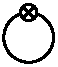
\includegraphics{frg/diagrams/FRG-wetterichEq-FS0_1_1.pdf}\end{gathered}\,,\label{eq:FS0}
\end{align}
starting with a \fs{} derivative \wrt{} the external (mean) field $\FSmf{\FSsf} {}_{\FSidxE{u}}$ we arrive at the flow equation for the one-point function
\begin{align}
	\cm{2,\FSvertexDt{\FSidxE{u}}}
	%FRG`wetterichEq`FS1[{2, {3, 1}}][[1]]
	=-\cm{\FSc{\FSidxE{u},\FSidxI{a},\FSidxI{c},\FSidxI{c}},\ncm{\FSpropagator{\FSidxI{a},\FSidxI{b}},\FSvertex{\FSidxI{b},\FSidxE{u},\FSidxI{c}},\FSpropagator{\FSidxI{c},\FSidxI{d}},\FSregulatorDt{\FSidxI{d},\FSidxI{a}}}}
	=-\cm{\FSc{\FSidxE{u},\FSidxI{a},\FSidxI{c},\FSidxI{c}}}\,\begin{gathered}\includegraphics{frg/diagrams/FRG-wetterichEq-FS1_231_1.pdf}\end{gathered}\,.\label{eq:FS1}
\end{align}
An additional \fs{} derivative \wrt{} the external (mean) field $\FSmf{\FSsf} {}_{\FSidxE{v}}$ of \cref{eq:FS1} leads to the flow equation of the two-point function
\begin{align}
	\cm{2,\FSvertexDt{\FSidxE{v},\FSidxE{u}}}
	%*** Combinatorics
	&=\, \skeleton{T_{2,2}} + \skeleton{T_{2,1}} \,=\, \skeleton{2} + \skeleton{1} \label{eq:FS2}
	%*** FS expressions
	\newSubEqBlock\\[.25em]
	%FRG`wetterichEq`FS2[{3, {3, 2}}][[1]]
	&= \cm{\FSc{\FSidxE{u},\FSidxI{a},\FSidxE{v},\FSidxI{a},\FSidxI{c},\FSidxI{c},\FSidxI{e},\FSidxI{e}},\ncm{\FSpropagator{\FSidxI{a},\FSidxI{b}},\FSvertex{\FSidxI{b},\FSidxE{v},\FSidxI{c}},\FSpropagator{\FSidxI{c},\FSidxI{d}},\FSvertex{\FSidxI{d},\FSidxE{u},\FSidxI{e}},\FSpropagator{\FSidxI{e},\FSidxI{f}},\FSregulatorDt{\FSidxI{f},\FSidxI{a}}}} +  \subEqTag \label{eq:FS2_332_1}\\[.25em]
	%FRG`wetterichEq`FS2[{3, {3, 2}}][[2]]
	&\qquad + \cm{\FSc{\FSidxE{u},\FSidxE{v},\FSidxE{u},\FSidxI{a},\FSidxE{v},\FSidxI{a},\FSidxI{c},\FSidxI{c},\FSidxI{e},\FSidxI{e}},\ncm{\FSpropagator{\FSidxI{a},\FSidxI{b}},\FSvertex{\FSidxI{b},\FSidxE{u},\FSidxI{c}},\FSpropagator{\FSidxI{c},\FSidxI{d}},\FSvertex{\FSidxI{d},\FSidxE{v},\FSidxI{e}},\FSpropagator{\FSidxI{e},\FSidxI{f}},\FSregulatorDt{\FSidxI{f},\FSidxI{a}}}} - \subEqTag \label{eq:FS2_332_2}\\[.25em]
	%FRG`wetterichEq`FS2[{2, {4, 1}}][[1]]
	&\qquad -\cm{\FSc{\FSidxE{u},\FSidxI{a},\FSidxE{v},\FSidxI{a},\FSidxI{c},\FSidxI{c}},\ncm{\FSpropagator{\FSidxI{a},\FSidxI{b}},\FSvertex{\FSidxI{b},\FSidxE{v},\FSidxE{u},\FSidxI{c}},\FSpropagator{\FSidxI{c},\FSidxI{d}},\FSregulatorDt{\FSidxI{d},\FSidxI{a}}}} \subEqTag \label{eq:FS2_241_1}
	\newSubEqBlockPrime\\[.25em]
	%*** Diagrams
	&=\cm{\FSc{\FSidxE{u},\FSidxI{a},\FSidxE{v},\FSidxI{a},\FSidxI{c},\FSidxI{c},\FSidxI{e},\FSidxI{e}}}\,\begin{gathered}\includegraphics{frg/diagrams/FRG-wetterichEq-FS2_332_1.pdf}\end{gathered} + \subEqTagPrime \label{eq:FS2_332_1-diagram}\\
	&\qquad +\cm{\FSc{\FSidxE{u},\FSidxE{v},\FSidxE{u},\FSidxI{a},\FSidxE{v},\FSidxI{a},\FSidxI{c},\FSidxI{c},\FSidxI{e},\FSidxI{e}}}\,\begin{gathered}\includegraphics{frg/diagrams/FRG-wetterichEq-FS2_332_2.pdf}\end{gathered} - \subEqTagPrime \label{eq:FS2_332_2-diagram}\\
	&\qquad -\cm{\FSc{\FSidxE{u},\FSidxI{a},\FSidxE{v},\FSidxI{a},\FSidxI{c},\FSidxI{c}}}\,\begin{gathered}\includegraphics{frg/diagrams/FRG-wetterichEq-FS2_241_1.pdf}\end{gathered}\,. \subEqTagPrime \label{eq:FS2_241_1-diagram}
\end{align}
Computing flow equations for higher-order \nptFunctions{} beyond $n=2$ is in principle straight forward, but the number of involved diagrams grows rapidly making a computation by hand error prone and at some point simply unfeasible.
Packages like \textit{DoFun}~\cite{Huber:2019dkb,DoFun:GitHub} or \textit{QMeS-Derivation}~\cite{Pawlowski:2021tkk,QMeS:GitHub} can be used to automate this process using the computer algebra system \WAMwR.
We use our own \WAM{} code~\cite{Steil:2023PhDFlowEquationsNB} for such and related diagrammatic computations.
The expressions and diagrams in \cref{eq:FS1,eq:FS2,eq:FS3,eq:FS4} have been programmatically generated with our \WAM{} code~\cite{Steil:2023PhDFlowEquationsNB} and exported to \LaTeX{} using propose build export methods.
The diagrams have been programmatically generated and rendered using \textit{Axodraw Version 2}~\cite{Collins:2016aya}.
In the following \cref{eq:FS3,eq:FS4} we present the flow equations for the three- and four-point functions in a skeletonized form\footnote{%
	Following the convention introduced in \cref{sec:compactNotations} we use $\skeleton{n}$ to represent a sequence of $n$ omitted elements.
	$\FScSkeleton{}{n}{}$ are abbreviated \fs{} sign factors, see \cref{eq:FScDef,eq:FScAbr} and the related discussion in \cref{app:FS}.
	$\skeleton{T_{n,k}}$ represents the number of diagrams of a specific type, see \cref{tab:FScombinatorics} and the related discussion.
	
} presenting mainly the classes of involved diagrams.
The flow of the three-point function is governed by
\begin{align}
	\cm{2,\FSvertexDt{\FSidxE{w},\FSidxE{v},\FSidxE{u}}}
	%*** Combinatorics
	&=\, \skeleton{T_{3,3}} + \skeleton{T_{3,2}} + \skeleton{T_{3,1}}\,=\, \skeleton{6} + \skeleton{6} + \skeleton{1} \label{eq:FS3}
	%*** FS expressions
	\newSubEqBlock\\[.25em]
	%FRG`wetterichEq`FS3[{4, {3, 3}}][[1]]
	&= -\cm{\FScSkeleton{}{6}{},\ncm{\FSpropagator{\FSidxI{a},\FSidxI{b}},\FSvertex{\FSidxI{b},\FSidxE{w},\FSidxI{c}},\FSpropagator{\FSidxI{c},\FSidxI{d}},\FSvertex{\FSidxI{d},\FSidxE{v},\FSidxI{e}},\FSpropagator{\FSidxI{e},\FSidxI{f}},\FSvertex{\FSidxI{f},\FSidxE{u},\FSidxI{g}},\FSpropagator{\FSidxI{g},\FSidxI{h}},\FSregulatorDt{\FSidxI{h},\FSidxI{a}}}}+\skeleton{5} +  \subEqTag \label{eq:FS3_433_1}\\[.25em]
	%FRG`wetterichEq`FS3[{3, {3, 1}, {4, 1}}][[1]]
	&\qquad + \cm{\FScSkeleton{}{5}{},\ncm{\FSpropagator{\FSidxI{a},\FSidxI{b}},\FSvertex{\FSidxI{b},\FSidxE{w},\FSidxI{c}},\FSpropagator{\FSidxI{c},\FSidxI{d}},\FSvertex{\FSidxI{d},\FSidxE{v},\FSidxE{u},\FSidxI{e}},\FSpropagator{\FSidxI{e},\FSidxI{f}},\FSregulatorDt{\FSidxI{f},\FSidxI{a}}}}+\skeleton{5} - \subEqTag \label{eq:FS3_33141_1}\\[.25em]
	%FRG`wetterichEq`FS3[{2, {5, 1}}][[1]]
	&\qquad -\cm{\FScSkeleton{}{4}{},\ncm{\FSpropagator{\FSidxI{a},\FSidxI{b}},\FSvertex{\FSidxI{b},\FSidxE{w},\FSidxE{v},\FSidxE{u},\FSidxI{c}},\FSpropagator{\FSidxI{c},\FSidxI{d}},\FSregulatorDt{\FSidxI{d},\FSidxI{a}}}} \subEqTag \label{eq:FS3_251_1}
	\newSubEqBlockPrime\\[.25em]
	%*** Diagrams
	&=-\cm{\FScSkeleton{}{6}{}}\,\begin{gathered}\includegraphics{frg/diagrams/FRG-wetterichEq-FS3_433_1.pdf}\end{gathered}+\skeleton{5} + \subEqTagPrime \label{eq:FS3_433_1-diagram}\\
	&\qquad +\cm{\FScSkeleton{}{5}{}}\,\begin{gathered}\includegraphics{frg/diagrams/FRG-wetterichEq-FS3_33141_1.pdf}\end{gathered}+\skeleton{5} - \subEqTagPrime \label{eq:FS3_33141_1-diagram}\\
	&\qquad -\cm{\FScSkeleton{}{4}{}}\,\begin{gathered}\includegraphics{frg/diagrams/FRG-wetterichEq-FS3_251_1.pdf}\end{gathered}\,, \subEqTagPrime \label{eq:FS3_251_1-diagram}
\end{align}
and the flow of the four-point function follows as
\begin{align}
	\cm{2,\FSvertexDt{\FSidxE{x},\FSidxE{w},\FSidxE{v},\FSidxE{u}}}
	%*** Combinatorics
	&=\, \skeleton{T_{4,4}} + \skeleton{T_{4,3}} + (\skeleton{T_{4,2}}) + \skeleton{T_{4,1}} \,= \notag\\
	&=\, \skeleton{24} + \skeleton{36} + (\skeleton{8} + \skeleton{6}) + \skeleton{1}\label{eq:FS4}
	%*** FS expressions
	\newSubEqBlock\\[.25em]
	%FRG`wetterichEq`FS4[{5, {3, 4}}][[1]]
	&= \cm{\FScSkeleton{}{8}{},\ncm{\FSpropagator{\FSidxI{a},\FSidxI{b}},\FSvertex{\FSidxI{b},\FSidxE{x},\FSidxI{c}},\FSpropagator{\FSidxI{c},\FSidxI{d}},\FSvertex{\FSidxI{d},\FSidxE{w},\FSidxI{e}},\FSpropagator{\FSidxI{e},\FSidxI{f}},\FSvertex{\FSidxI{f},\FSidxE{v},\FSidxI{g}},\FSpropagator{\FSidxI{g},\FSidxI{h}},\FSvertex{\FSidxI{h},\FSidxE{u},\FSidxI{i}},\FSpropagator{\FSidxI{i},\FSidxI{j}},\FSregulatorDt{\FSidxI{j},\FSidxI{a}}}}+\skeleton{23} -  \subEqTag \label{eq:FS4_534_1}\\[.25em]
	%FRG`wetterichEq`FS4[{4, {3, 2}, {4, 1}}][[1]]
	&\qquad -\cm{\FScSkeleton{}{7}{},\ncm{\FSpropagator{\FSidxI{a},\FSidxI{b}},\FSvertex{\FSidxI{b},\FSidxE{x},\FSidxI{c}},\FSpropagator{\FSidxI{c},\FSidxI{d}},\FSvertex{\FSidxI{d},\FSidxE{w},\FSidxI{e}},\FSpropagator{\FSidxI{e},\FSidxI{f}},\FSvertex{\FSidxI{f},\FSidxE{v},\FSidxE{u},\FSidxI{g}},\FSpropagator{\FSidxI{g},\FSidxI{h}},\FSregulatorDt{\FSidxI{h},\FSidxI{a}}}}+\skeleton{35} + \subEqTag \label{eq:FS4_43241_1}\\[.25em]
	%FRG`wetterichEq`FS4[{3, {3, 1}, {5, 1}}][[1]]
	&\qquad + \Big(\cm{\FScSkeleton{}{6}{},\ncm{\FSpropagator{\FSidxI{a},\FSidxI{b}},\FSvertex{\FSidxI{b},\FSidxE{x},\FSidxI{c}},\FSpropagator{\FSidxI{c},\FSidxI{d}},\FSvertex{\FSidxI{d},\FSidxE{w},\FSidxE{v},\FSidxE{u},\FSidxI{e}},\FSpropagator{\FSidxI{e},\FSidxI{f}},\FSregulatorDt{\FSidxI{f},\FSidxI{a}}}}+\skeleton{7} + \subEqTag \label{eq:FS4_33151_1}\\[.25em]
	%FRG`wetterichEq`FS4[{3, {4, 2}}][[1]]
	&\qquad\qquad\quad + \cm{\FScSkeleton{}{6}{},\ncm{\FSpropagator{\FSidxI{a},\FSidxI{b}},\FSvertex{\FSidxI{b},\FSidxE{x},\FSidxE{w},\FSidxI{c}},\FSpropagator{\FSidxI{c},\FSidxI{d}},\FSvertex{\FSidxI{d},\FSidxE{v},\FSidxE{u},\FSidxI{e}},\FSpropagator{\FSidxI{e},\FSidxI{f}},\FSregulatorDt{\FSidxI{f},\FSidxI{a}}}}+\skeleton{5}\Big) - \subEqTag \label{eq:FS4_342_1}\\[.25em]
	%FRG`wetterichEq`FS4[{2, {6, 1}}][[1]]
	&\qquad -\cm{\FScSkeleton{}{5}{},\ncm{\FSpropagator{\FSidxI{a},\FSidxI{b}},\FSvertex{\FSidxI{b},\FSidxE{x},\FSidxE{w},\FSidxE{v},\FSidxE{u},\FSidxI{c}},\FSpropagator{\FSidxI{c},\FSidxI{d}},\FSregulatorDt{\FSidxI{d},\FSidxI{a}}}} \subEqTag \label{eq:FS4_261_1}
	\newSubEqBlockPrime\\[.25em]
	%*** Diagrams
	&=\cm{\FScSkeleton{}{8}{}}\,\begin{gathered}\includegraphics{frg/diagrams/FRG-wetterichEq-FS4_534_1.pdf}\end{gathered}+\skeleton{23} - \subEqTagPrime \label{eq:FS4_534_1-diagram}\\
	&\qquad -\cm{\FScSkeleton{}{7}{}}\,\begin{gathered}\includegraphics{frg/diagrams/FRG-wetterichEq-FS4_43241_1.pdf}\end{gathered}+\skeleton{35} + \subEqTagPrime \label{eq:FS4_43241_1-diagram}\\
	&\qquad +\Big(\cm{\FScSkeleton{}{6}{}}\,\begin{gathered}\includegraphics{frg/diagrams/FRG-wetterichEq-FS4_33151_1.pdf}\end{gathered}+\skeleton{7} + \subEqTagPrime \label{eq:FS4_33151_1-diagram}\\
	&\qquad\qquad\quad +\cm{\FScSkeleton{}{6}{}}\,\begin{gathered}\includegraphics{frg/diagrams/FRG-wetterichEq-FS4_342_1.pdf}\end{gathered}+\skeleton{5}\Big) - \subEqTagPrime \label{eq:FS4_342_1-diagram}\\
	&\qquad -\cm{\FScSkeleton{}{5}{}}\,\begin{gathered}\includegraphics{frg/diagrams/FRG-wetterichEq-FS4_261_1.pdf}\end{gathered}\,. \subEqTagPrime \label{eq:FS4_261_1-diagram}
\end{align}

A common way to reduce the number of diagrams, which only differ by the location of the regulator insertion in the loop, is to introduce the \rgtime{}/scale derivative $\tilde{\partial}_t$ ($\tilde{\partial}_k$) which only acts on the regulator, see, \eg{}, \ccite{DoFun:GitHub}.
This allows for a unification of certain diagrams using
\begin{align}
\tilde{\partial}_t \FSpropagator{\FSidx{a},\FSidx{b}}[\FSmf{\FSsf}] &= - \FSc{\FSidx{b},\FSidx{b}} \FSpropagator{\FSidx{a},\FSidx{m}}[\FSmf{\FSsf}] \FSregulatorDt{\FSidx{m},\FSidx{n}} \FSpropagator{\FSidx{n},\FSidx{b}}[\FSmf{\FSsf}]\, ,
\label{eq:dtTildeG}
\end{align}
which follows directly from the implicit definition \eqref{eq:GkabImplicit} of the propagator.
Using \cref{eq:dtTildeG} to simplify, \ie{}, reduce the number of diagrams, in the flow \cref{eq:FS2,eq:FS3,eq:FS4} requires some care \wrt{} the involved signs and sign factors $(-1)^{\ldots}$. In the following we use $\tilde{\partial}_t$ ($\tilde{\partial}_k$) only for schematic discussions and to simplify final expressions after all traces in field and internal spaces have been performed.

\FloatBarrier%
We conclude this subsection with a remark on the involved combinatorics \dash{} diagrammatic complexity when computing flow equations for higher-order \nptFunctions{} in \fs{}.
The number of diagrams $B_n$ involved on the \rhs{} of a \frg{} flow equation for the \nptFunction{}  ${\protect\FSvertex{\protect\FSidx{x}_1,\ldots,\protect\FSidx{x}_n}}$ grows faster than $n!$.
It is given by the \ith{n} ordered Bell/Fubini number $B_n$~\cite{OEIS:A000670}
\begin{align}
	B_n&= \frac{1}{2}\Phi(\tfrac{1}{2},-n,0) =\sum_{k=1}^{n}T_{n,k} = \frac{1}{2\ln^{n+1}(2)}n!+\order((n-1)!)\, ,\label{eq:FSBn}
\end{align}
where the Triangle numbers $T_{n,k}$~\cite{OEIS:A019538} are given by
\begin{align}
	T_{n,k}&=k! S_n^{(k)}\, ,\label{eq:FSTnk}
\end{align}
with the Hurwitz-Lerch transcendent $\Phi$ and the Stirling number of the second kind $S_n^{(k)}$, see, \eg{}, \ccite{NIST:DLMF} Secs.~25.14 and 26.8.
In a combinatorics context $B_n$ is the ``number of preferential arrangements of $n$ labeled elements; or number of weak orders on n labeled elements; or number of ordered partitions of $[n]$''~\cite{OEIS:A000670}.
For a given $n$ and $k=n,\ldots,1$, $T_{n,k}$ represents the number of diagrams with $k$ vertices, which always have $k+1$ propagators, \cf{} \cref{eq:FS2,eq:FS3,eq:FS4}.
The asymptotic expansion in \cref{eq:FSBn} can be found in \ccite{Barthelemy1980Jan}.
The values of $B_n$ and $T_{n,k}$ for ${k=1,\ldots,n}$ and ${n=1,\ldots,6}$ are displayed in \cref{tab:FScombinatorics}. For further details regarding the underlying combinatorics/permutohedron, see, \eg{}, \ccite{SIMION1997149} p.~167ff and \ccite{Ziegler1995} p.~18ff.
Computing the full flow equations in \fs{} becomes extremely expensive/infeasible for larger $n$.
In this work we mainly study the flow equation for $\FSvertex{}$ itself, with \cref{subsec:0dSU2flowEqs,sec:gnInfInhomo} as the most notable exceptions.
\clearpage
\begin{table}[t]
	\centering
	\caption{\label{tab:FScombinatorics}%
		Number of field space diagrams $B_n$ on the \rhs{} of the flow equation ${\protect\FSvertexDt{\protect\FSidxE{x}_1,\ldots,\protect\FSidxE{x}_n}}$ for ${n=1,\ldots,6}$.
		$T_{n,k}$ diagrams with $k+1$ propagators for ${k=1,\ldots,n}$ contribute to $B_n$ for a given $n$. $B_n$ is given by \cref{eq:FSBn} while $T_{n,k}$ is given by \cref{eq:FSTnk}.
		The factors for $n=2,\ldots,4$ appear in \cref{eq:FS2,eq:FS3,eq:FS4} as $\skeleton{T_{n,k}}$ and $\skeleton{T_{n,k}-1}$ in respective subequations.
	}% Why the protect: [https://tex.stackexchange.com/a/12699/]
	\vspace{\TableAbovecaptionskip}
	\renewcommand{\arraystretch}{1.15}
	\begin{tabular}{l | c  c c c c c || c}
		\toprule
		$T_{n,k} $& $k=1$ & $k=2$ & $k=3$ & $k=4$ & $k=5$ & $k=6$ & $B_n$ \\\midrule
		$n=1$ & $1$ & 	 & 	 & 	 & 	 & 	 & $1$ \\
		$n=2$ & $1$ & $2$ & 	 & 	 & 	 & 	 & $3$ \\
		$n=3$ & $1$ & $6$ & $6$ & 	 & 	 & 	 & $13$ \\
		$n=4$ & $1$ & $14$ & $36$ & $24$ & 	 & 	 & $75$ \\
		$n=5$ & $1$ & $30$ & $150$ & $240$ & $120$ & 	 & $541$ \\
		$n=6$ & $1$ & $62$ & $540$ & $1560$ & $1800$ & $720$ & $4683$ \\
		\bottomrule
	\end{tabular}
\end{table}

\subsection{Renormalization group consistency}\label{subsec:RGconsistency}
In this subsection we discuss the concept of \textit{renormalization group consistency} with focus on the \frg{} framework following the excellent discussion of \ccite{Braun:2018svj}.
Additional information can be found in \ccite{Braun:2003ii,Herbst:2013ufa,Springer2017,Leonhardt:2019mpy,PhysRevD.87.076004}.
In the context of the \frg{} the question of \rgcy{} is closely related to the appropriate choice of \uv{} initial scale $\Lambda$ and corresponding initial action $S_\Lambda$, \cf{} \cref{subsubsec:regulator}.
For a given theory with classical action $S$ the \frg{} provides both a renormalization and regularization scheme based on the \eaa{} $\FSeaa_k$.
The Wetterich equation can be used to study the \rgscale{} evolution of the \eaa{} $\FSeaa_k$ connecting the microscopic action $S$ of the theory at hand to the full quantum \ea{} $\Gamma_\mathrm{1PI}$. 
This process however requires an initialization of the Wetterich equation at an \uv{} initial scale $\Lambda$.
The introduction of such a scale and corresponding regularization, which the regulator provides in the \eaa{} $\FSeaa_k$, is a computational necessity.
Physical observables encoded in $\FSeaa_0[\FSsf]=\Gamma_\mathrm{1PI}[\FSsf]\equiv\Gamma[\FSsf]$ and its moments however should not depend on the scale $\Lambda$:
\begin{align}
	\Lambda\dod{\Gamma[\FSsf]}{\Lambda}\equiv \Lambda\dod{\FSeaa_0[\FSsf]}{\Lambda}\overset{!}{=} 0\,.
	\label{eq:rgcCondition}
\end{align}
This seemingly simple requirement is the governing equation for a consistent regularization and renormalization of a given theory~\cite{Braun:2018svj}.
\Cref{eq:rgcCondition} is called \textit{RG consistency condition} and a computation of $\Gamma[\FSsf]$ for a given theory is considered \textit{RG-consistent} \ifandonlyif{} the condition \nolinebreak[3]\eqref{eq:rgcCondition} is met.
In the \frg{} framework we can translate this requirement for the \ir{} \eaa{} $\FSeaa_0[\FSsf]$ to non-zero $k$ by integrating the \frgEquation{} from the \uv{} $k=\Lambda$ down to $k<\Lambda$\footnote{%
	Due to our convention \eqref{eq:def_rg_time} for \rgtime{}, \cref{eq:rgcWetterichEqInt} and subsequent expressions differ from the corresponding ones in \ccite{Braun:2018svj}, see, \eg{}, Eq. (11a) of \ccite{Braun:2018svj}, involving the \frg{} flux $\FRGflow_{k}[\FSsf]$ by a sign.%
}
\begin{align}
	\FSeaa_k[\FSsf]&= \FSeaa_\Lambda[\FSsf] -\int_\Lambda^k \frac{\dif k'}{k'} \FRGflow_{k'}[\FSsf]\,.
	\label{eq:rgcWetterichEqInt}
\end{align}
By taking a derivative of \cref{eq:rgcWetterichEqInt} \wrt{} $\Lambda$ and evaluating the subsequent expression at ${k=0}$ and an arbitrary ${k\neq\Lambda}$ we obtain
\begin{subequations}\label{eq:rgc}
\begin{align}
	\Lambda\dod{\FSeaa_0[\FSsf]}{\Lambda}&=\Lambda\dod{\FSeaa_\Lambda[\FSsf]}{\Lambda}+\FRGflow_{\Lambda}[\FSsf]\label{eq:rgc0}\,,\\
	\Lambda\dod{\FSeaa_k[\FSsf]}{\Lambda}&=\Lambda\dod{\FSeaa_\Lambda[\FSsf]}{\Lambda}+\FRGflow_{\Lambda}[\FSsf]\label{eq:rgck}\,.
\end{align}
\end{subequations}
Using the \rgcy{} condition \eqref{eq:rgcCondition} with \cref{eq:rgc0} and equating it with \cref{eq:rgck}, we obtain a \rgcy{} condition for any $k\neq \Lambda$
\begin{align}
	0\overset{!}{=} \Lambda\dod{\FSeaa_0[\FSsf]}{\Lambda} =\Lambda\dod{\FSeaa_\Lambda[\FSsf]}{\Lambda}+\FRGflow_{\Lambda}[\FSsf]= \Lambda\dod{\FSeaa_k[\FSsf]}{\Lambda}\, .
	\label{eq:rgcConditionUV}
\end{align}
The included statement $0=\Lambda\partial_\Lambda\FSeaa_\Lambda[\FSsf]+\FRGflow_{\Lambda}[\FSsf]$ in \cref{eq:rgcConditionUV} dictates that \rgcy{} is realized in the \frg{} approach if the \ic{}
$\FSeaa_\Lambda[\FSsf]$ changes with $\Lambda$ according to the \frg{} flux $\FRGflow_{\Lambda}[\FSsf]$ at the initial scale.
The latter is an immensely powerful and practically useful statement and merits further elaboration.

\subsubsection{Construction of RG consistent initial conditions}\label{subsubsec:rgcICS}
Lets first consider a scenario where $\Lambda$ can be chosen asymptotically large in the sense that
\begin{align}
	\forall s_i\in s \quad \frac{s_i}{\Lambda}\ll 1\, ,\label{eq:rgcScales}
\end{align}
with the set $s$ which includes all mass scales of the theory at hand.
This set consists of all intrinsic mass scales $m_\phys$, \eg{}, particle masses and decay widths, and external scales $m_\ext$, \eg{}, temperature $T$ or chemical potential $\mu$.
If $\Lambda$ is indeed asymptotically large compared to those scales, the initial action $\FSeaa_\Lambda[\FSsf]=S[\FSsf]$ can be considered classical in the sense that the \frg{} flux $\FRGflow_{\Lambda}[\FSsf]$ at the initial scale vanishes since all fluctuations are included in $\FSeaa_\Lambda[\FSsf]$.
This entails initial-scale-independence of the \ic{} $\Lambda\partial_\Lambda\FSeaa_\Lambda[\FSsf]=\Lambda\partial_\Lambda S[\FSsf]=0$.
Such situations with asymptotically large initial scale in the sense of \cref{eq:rgcScales} will be studied in \cref{chap:zeroONSU2,chap:GN}.\bigskip

\fullWidthFigure%
	{frg/figures/rg_consistency.pdf}% Graphics
	[]% Sublabels
	{%
		Schematic \frg{} flow \dash{} \rgscaleevolution{} of the \eaa{} in the space of its couplings $\{\lambda_i\}$ \dash{} (in blue and red) from the \uv{} initial condition $\FSeaa_\Lambda$ towards the \ir{} at differing external parameter sets $m_\ext^{(0)}\neq m_\ext^{(1)}$.
		The red-dashed line represents a \rg{} inconsistent flow at $m_\ext^{(1)}$ starting from $\FSeaa_{\Lambda'}^{(0)}$ and not ending at the correct \ir{} result $\FSeaa_{0}^{(1)}$.
		For readability in the figure we abbreviated $\FSeaa_k^{(0)}\equiv\FSeaa_k[\FSsf;m_\ext^0]$ and $\FSeaa_k^{(1)}\equiv\FSeaa_k[\FSsf;m_\ext^1]$.%
	}%Caption
	{fig:frg_rg_consistency}%Label
In certain applications \dash{} prominently when working with \loefts{} of \qcd{}, \cf{} \cref{sec:qcdModels,chap:QMM} \dash{} choosing an asymptotically large $\Lambda$ for a given classical action $S$ is conceptually not feasible and in some cases even mathematically impossible.
In those cases it is possible to use \rgcy{} as a construction principle for a \rgscaledependent{} \ic{} $\FSeaa_\Lambda[\FSsf]=S_\Lambda[\FSsf]$ in the following way.

Consider a \loeft{} for which we specify the action ${\FSeaa_\LambdaP[\FSsf;m_\ext^0]=S[\FSsf]}$ at an intermediate scale $\LambdaP$ with/at a corresponding set of physical parameters $m_\phys^0$/ external scales $m_\ext^0$.
Here $m_\ext^0$ is typically (but not necessarily) the vacuum, \eg{}, $T=\mu=0$, and  $m_\phys^0$ a set of \ir{} observables realized by properly chosen couplings in $\FSeaa_\LambdaP[\FSsf]$.
In this scenario $\LambdaP$ can not be considered as asymptotically large in the sense of \cref{eq:rgcScales} and thus $\FSeaa_\LambdaP[\FSsf]$ does not include all relevant fluctuations especially \wrt{} fluctuations related to external scales $m_\ext$ beyond $m_\ext^0$, \eg{}, thermal and density fluctuations beyond the vacuum.
$\FSeaa_\LambdaP[\FSsf;m_\ext^0]$ is therefore not suited for computations at $m_\ext^1\neq m_\ext^0$.
To remedy these situations and to enable \rgct{} computations at differing external scales $m_\ext^1\neq m_\ext^0$ one can use the Wetterich equation~\eqref{eq:rgcWetterichEqInt} to reconstruct an \uv{} initial action $\FSeaa_\Lambda[\FSsf;m_\ext^0]$ at a higher, proper \uv{} initial scale $\Lambda>\LambdaP$:
\begin{align}
	S_\Lambda[\FSsf]\equiv\FSeaa_\Lambda[\FSsf;m_\ext^0]&= \FSeaa_\LambdaP[\FSsf;m_\ext^0] +\int_\Lambda^\LambdaP \frac{\dif k'}{k'} \FRGflow_{k'}[\FSsf;m_\ext^0]\,.
	\label{eq:rgcEq14}
\end{align}
$S_\Lambda[\FSsf]$ includes \rgscaledependent{} counter terms \dash{} corrections to $S[\FSsf]$ \dash{} generated by the \frg{} flux $\FRGflow_{k}[\FSsf;m_\ext^0]$ to ensure \rgcy{} $\Lambda\partial_\Lambda\FSeaa_0[\FSsf]=0$ by guaranteeing $\Lambda\partial_\Lambda \FSeaa_\Lambda[\FSsf;m_\ext^0] = -\FRGflow_{\Lambda}[\FSsf;m_\ext^0]$ while maintaining $\FSeaa_\LambdaP[\FSsf;m_\ext^0]=S[\FSsf]$. 
Therefore guaranteeing an unchanged $\FSeaa_k[\FSsf;m_\ext^0]$ for $k<\LambdaP$ by construction, since \cref{eq:rgcWetterichEqInt} at $m_\ext^0$ and \cref{eq:rgcEq14} entail
\begin{subequations}\label{eq:rgcEq15}
\begin{align}
	\FSeaa_k[\FSsf;m_\ext^0]&= \FSeaa_\LambdaP[\FSsf;m_\ext^0] -\int_\LambdaP^k \frac{\dif k'}{k'} \FRGflow_{k'}[\FSsf;m_\ext^0]\label{eq:rgcEq15a}\\
	&=\FSeaa_\Lambda[\FSsf;m_\ext^0] -\int_\Lambda^k \frac{\dif k'}{k'} \FRGflow_{k'}[\FSsf;m_\ext^0]\label{eq:rgcEq15n}\, .
\end{align}
\end{subequations}
$S_\Lambda[\FSsf]$ represents an \uv{} completion of the \loeft{} specified at $\LambdaP$ with ${\FSeaa_\LambdaP[\FSsf;m_\ext^0]=S[\FSsf]}$.
This construction is visualized in \cref{fig:frg_rg_consistency} in blue.

By reconstructing $S_\Lambda[\FSsf]\equiv\FSeaa_\Lambda[\FSsf;m_\ext^0]$ up to a scale $\Lambda$, which can be considered as asymptotically large in the sense of \cref{eq:rgcScales}, we can ensure that a change in external parameters leaves the regularization and renormalization encoded in the running of $S_\Lambda[\FSsf]$ unchanged:
\begin{align}
	\dod{}{m_\ext}\!\sbr{\Lambda\dod{S_\Lambda[\FSsf]}{\Lambda}}=0\,.
	\label{eq:rgcEq3} 
\end{align}
In other words $S_\Lambda[\FSsf]$ is suited for computations at $m_\ext^1\neq m_\ext^0$ since $\Lambda\gg m_\ext$ and $\FRGflow_{\Lambda}[\FSsf;m_\ext^0]=\FRGflow_{\Lambda}[\FSsf;m_\ext^1]$.
Integrating \cref{eq:rgcEq3} from $m_\ext^0$ to $m_\ext^1$ we obtain
\begin{align}
	\Lambda\dod{S_\Lambda[\FSsf]}{\Lambda} \equiv \Lambda\dod{\FSeaa_\Lambda[\FSsf;m_\ext^0]}{\Lambda} = \Lambda\dod{\FSeaa_\Lambda[\FSsf;m_\ext^1]}{\Lambda}\,.
	\label{eq:rgcEq3int}
\end{align}
Note that $\FSeaa_\Lambda[\FSsf;m_\ext^1]=\FSeaa_\Lambda[\FSsf;m_\ext^0]$ is not necessary: an explicit dependence of $S_\Lambda[\FSsf]$ on $m_\ext$ is possible\footnote{
	Certain \loefts{} can require counter terms in $S_\Lambda[\FSsf]$, which depend on $m_\ext$ explicitly, see, \eg{}, Sec.~III.B of \nbccite{Braun:2018svj} for an explicit example involving diquarks and chemical potential in the context of \loefts{} for \qcd{}.%
} as long as \cref{eq:rgcEq3int} holds.
In \cref{fig:frg_rg_consistency} and our applications in \cref{chap:QMM} we consider $S_\Lambda[\FSsf]$ without an explicit dependence on $m_\ext$.
Using the Wetterich equation \eqref{eq:rgcWetterichEqInt} at $m_\ext^1$ with \cref{eq:rgcEq14}, we can construct a \rgcy{} condition at $m_\ext^1\neq m_\ext^0$:
\begin{subequations}\label{eq:rgcm}
\begin{align}
	0&\overset{!}{=} \Lambda\dod{\FSeaa_0[\FSsf;m_\ext^1]}{\Lambda} =\Lambda\dod{\FSeaa_k[\FSsf;m_\ext^1]}{\Lambda}= \Lambda\dod{\FSeaa_\Lambda[\FSsf;m_\ext^1]}{\Lambda} + \FRGflow_{\Lambda}[\FSsf;m_\ext^1]\, ,\label{eq:rgcm1p}\\
	0&\overset{!}{=}\Lambda\dod{\FSeaa_0[\FSsf;m_\ext^1]}{\Lambda} = \FRGflow_{\Lambda}[\FSsf;m_\ext^1]-\FRGflow_{\Lambda}[\FSsf;m_\ext^0]\label{eq:rgcm1}\, ,
\end{align}
\end{subequations}
where we used \cref{eq:rgcEq3int} in \cref{eq:rgcm1p} to obtain \cref{eq:rgcm1}.
The latter can be used to conveniently define applicability ranges $\Lambda[m_\ext^1]$, where $\Lambda[m_\ext^1]$ is the range/scale for which \cref{eq:rgcm1} holds to a given accuracy~\cite{Braun:2018svj}.
Using $S_\Lambda[\FSsf]$ as an \ic{} for a large range of external parameters $m_\ext$ by guaranteeing \cref{eq:rgcm1} (to a chosen accuracy), we note that at $k=\LambdaP$
\begin{align}
	\FSeaa_\LambdaP[\FSsf;m_\ext^1]&= \FSeaa_\LambdaP[\FSsf;m_\ext^0] -\int_\Lambda^\LambdaP \frac{\dif k'}{k'} \del{\FRGflow_{k'}[\FSsf;m_\ext^1]-\FRGflow_{k'}[\FSsf;m_\ext^0]}\,,
	\label{eq:rgcSLambdaPmext1}
\end{align}
where we again used the Wetterich equation \eqref{eq:rgcWetterichEqInt} with \cref{eq:rgcEq14}.
$\FSeaa_\LambdaP[\FSsf;m_\ext^1]$ differs from the specified action $\FSeaa_\LambdaP[\FSsf;m_\ext^0]=S[\FSsf]$ by the fluctuations associated with $m_\ext$.
The latter are incorporated by integrating the difference of \frg{} fluxes $\FRGflow_{k'}[\FSsf;m_\ext^1]-\FRGflow_{k'}[\FSsf;m_\ext^0]$ from $\Lambda$ to $\LambdaP$, \cf{} \cref{fig:frg_rg_consistency}.
It is imperative to include those fluctuations at $k=\LambdaP$ and $\FSeaa_\LambdaP[\FSsf;m_\ext^0]=S[\FSsf]$ alone is not suited for a flow at $m_\ext^1$ \dash{} a situation illustrated in \cref{fig:frg_rg_consistency} in red.\bigskip

To conclude this section we want to comment on some practical limitations when leveraging the concept of \rgcy{}.
Throughout this section we frequently used the symbolically integrated Wetterich equation \eqref{eq:rgcWetterichEqInt} which is not a simple equation involving an ordinary integral.
The integrals in \cref{eq:rgcWetterichEqInt} and subsequent derived expressions are meant as solutions of the Wetterich equation, which are obtained by solving the differential equations associated with the \frg{} flux $\FRGflow_{k}[\FSsf]$.
Depending on the theory and truncation at hand this might be a rather involved process.
Furthermore \frg{} time integration \dash{} evolving the Wetterich equation in \rgscale{} from the \uv{} to the \ir{} \dash{} is for many theories and truncations irreversible.
This irreversibility is formally mentioned in the next \cref{subsec:RGflow} and discussed at length in \cref{chap:zeroONSU2} and especially in \cref{subsec:0dO1Entropy}.
Irreversibility makes the construction \eqref{eq:rgcEq14} of $S_\Lambda[\FSsf]\equiv\FSeaa_\Lambda[\FSsf;m_\ext^0]$ in the context of \loefts{} rather involved since a solution from the lower scale $\LambdaP$ up to $\Lambda>\LambdaP$ is practically/computationally not possible and
\begin{align}
	\FSeaa_\Lambda[\FSsf;m_\ext^0]-\int_\Lambda^\LambdaP \frac{\dif k'}{k'} \FRGflow_{k'}[\FSsf;m_\ext^0] &= \FSeaa_\LambdaP[\FSsf;m_\ext^0]\,
	\label{eq:rgcEq14rev}
\end{align}
would be the practical form of \eqref{eq:rgcEq14}:
$\FSeaa_\Lambda[\FSsf;m_\ext^0]$ has to be tuned such that $\FSeaa_\LambdaP[\FSsf;m_\ext^0]$ is recovered after flowing down from $\Lambda$ to $\LambdaP$. 
This presents an extremely difficult optimization problem, which might not even have (depending on the theory, truncation, and regulator employed) a solution for some explicit choices of $\FSeaa_\LambdaP[\FSsf;m_\ext^0]\equiv S[\FSsf]$.

That being said for some theories and truncations \frg{} time integration is reversible, \cf{} our large-$N$/mean-field studies in \cref{chap:GN,chap:QMM}, which simplifies the construction of suitable initial conditions $S_\Lambda[\FSsf]\equiv\FSeaa_\Lambda[\FSsf;m_\ext^0]$ immensely since direct computation of appropriate counter terms from the \cref{eq:rgcEq14} is possible and an optimization/tuning in the sense of \cref{eq:rgcEq14rev} is not required.

\subsection{Renormalization group equations as functional flow equations}\label{subsec:RGflow}
\begin{disclaimer}
	Parts of this subsection are based on the Secs.~II.B\dash{}C and IV.A of \nbccite{Koenigstein:2021syz}.
\end{disclaimer}
In the following we want to comment on the structure of the renormalization group equation for the \rgscaledependent{} generating functionals $Z_k[\FSff{J}]$, $W_k[\FSff{J}]$, and $\FSeaa_k[\FSmf{\FSsf}]$ for non-composite/non-scale-dependent fundamental fields $\FSfd{\FSsf}{a}\equiv\FSffd{\FSsf}{a}\Leftrightarrow \partial_t \FSfd{\FSsf}{a}=0$ and corresponding sources $\FSfd{J}{a}\equiv\FSffd{J}{a}$.
The evolution equation \eqref{eq:dWkdt} simplifies in this context to 
\begin{align}
	\dod{W_k[\FSff{J}]}{t}&=\dod{}{t}\ln Z_k[\FSff{J}]=\frac{1}{Z_k[\FSf{J}]}\dod{Z_k[\FSf{J}]}{t}
	= -\frac{1}{2}\partial_t \FSregulator{\FSidx{m},\FSidx{n}}\expectationValue{\FSffd{\FSsf}{n}\FSffd{\FSsf}{m}}{\FSff{J}}
	\label{eq:dWkdtnoscale}\,,
\end{align}
from which we can deduce the following evolution equations 
\begin{align}
	\dod{Z_k[\FSff{J}]}{t}&= -\frac{1}{2}\del{\partial_t \FSregulator{\FSidx{m},\FSidx{n}}}\frac{\delta}{\delta \FSmfu{J}{n}}\frac{\delta}{\delta \FSmfu{J}{m}} Z_{k}[\FSff{J}]
	= -\frac{1}{2}\del{\partial_t \FSregulator{\FSidx{m},\FSidx{n}}} Z_{k,\FSidx{n}\FSidx{m}}[\FSff{J}]\label{eq:dZkdtflow}\,,\\
	\dod{W_k[\FSff{J}]}{t}&= -\frac{1}{2}\del{\partial_t \FSregulator{\FSidx{m},\FSidx{n}}}\del[3]{ \frac{\delta}{\delta \FSmfu{J}{n}}\frac{\delta}{\delta \FSmfu{J}{m}} W_{k}[\FSff{J}] + \frac{\delta W_{k}[\FSff{J}]}{\delta \FSmfu{J}{n}}\frac{\delta W_{k}[\FSff{J}]}{\delta \FSmfu{J}{m}} }=\notag\\
	&= -\frac{1}{2}\del{\partial_t \FSregulator{\FSidx{m},\FSidx{n}}} \del[3]{W_{k,\FSidx{n}\FSidx{m}}[\FSff{J}]+W_{k,\FSidx{n}}[\FSff{J}]W_{k,\FSidx{m}}[\FSff{J}]}
	\label{eq:dWkdtflow}\,,
\end{align}
by rewriting the expectation value using the generating functionals.
The structure of \cref{eq:dZkdtflow} is that of a linear functional diffusion equation (\textit{heat equation})~\cite{Brydges:1987,Zumbach:1994kc,Rosten:2010vm,SkinnerScript,Salmhofer:2020Talk,Cannon:1984}, where $t$ corresponds to an effective temporal direction, while $\FSff{J}$ corresponds to an effective spatial direction.
Sometimes \cref{eq:dZkdtflow} is even explicitly denoted as a (non-linear) heat equation, \cf{} \cref{paragraph:HE}.
The regulator insertion $-\frac{1}{2}\partial_t \FSregulator{\FSidx{m},\FSidx{n}}$ acts as a diffusion coefficient contracted with the Hessian $Z_{k,\FSidx{n}\FSidx{m}}[\FSff{J}]$.
The \rgtime{} evolution of the generating functional $Z_k[\FSff{J}]$ is governed by the change \dash{} functional derivative $\delta/\delta{\FSffd{J}{n}}$ \dash{} of the functional gradient $Z_{k,\FSidx{m}}[\FSff{J}]$ weighted by the diffusion coefficient $-\frac{1}{2}\partial_t \FSregulator{\FSidx{m},\FSidx{n}}$.
The closely related evolution equation \eqref{eq:dWkdtflow} for $W_k[\FSff{J}]$ has a similar structure, but the Hessian $W_{k,\FSidx{n}\FSidx{m}}[\FSff{J}]$ gets modified by the product of two functional gradient terms $W_{k,\FSidx{n}}[\FSff{J}]W_{k,\FSidx{m}}[\FSff{J}]$.
The evolution equations for $Z_k[\FSff{J}]$ and $W_k[\FSff{J}]$ are due to their nature as functional diffusion equations \textit{flow equations}.

The \frgEquation{} 
\begin{align}
	\partial_t\FSeaa_k[\FSsf]
	%FRG`wetterichEq`FS0[{1}][[1]]
	=\frac{1}{2}\ncm{\FSpropagator{\FSidx{m},\FSidx{n}}[\FSsf],\FSregulatorDt{\FSidx{n},\FSidx{m}}}
	\equiv \FRGflow_k\sbr[1]{\mkern2mu\FSvertex{\FSidx{m},\FSidx{n}}[\FSmf{\FSsf}],\FSsf}\,,\label{eq:WetterichEqFlow}
\end{align}
does not manifest itself as a diffusion or flow equation at first glance. 
The \rhs{} of \cref{eq:WetterichEqFlow} depends non-linearly on the Hessian $\FSvertex{\FSidx{m},\FSidx{n}}[\FSmf{\FSsf}]$ through the propagator, \cf{} \cref{eq:GkabImplicit}, which prevents a direct interpretation as a linear functional diffusion equation.
Noting however that the \rhs{} of \cref{eq:WetterichEqFlow} does not depend on $\FSeaa_k[\FSsf]$ itself, we may consider the functional gradient $\FSvertex{\FSidx{a}}[\FSmf{\FSsf}]$ as the fundamental variable and by taking a corresponding functional derivative reformulate \cref{eq:WetterichEqFlow} as
\begin{align}
	\partial_t \FSvertex{\FSidx{a}}[\FSmf{\FSsf}] = \frac{\delta}{\delta \FSmfd{\FSsf}{a}}\FRGflow_k\sbr[1]{\mkern2mu\FSvertex{\FSidx{m},\FSidx{n}}[\FSmf{\FSsf}],\FSsf}\equiv\FRGflow_k^{,\FSidx{a}}\sbr[1]{\mkern2mu\FSvertex{\FSidx{m},\FSidx{n}}[\FSmf{\FSsf}],\FSsf}\,,
	\label{eq:dWetterichEqFlow}
\end{align}
which has the form of a functional convection\footnote{
	In the following we use the term \textit{convection} in the fluid-dynamical sense as a phenomenon including both \textit{advection} and \textit{diffusion}.
	For more details on those terms we refer to \cref{sec:conservationLaws}.%
} equation~\cite{Koenigstein:2021syz,Grossi:2019urj}.
The \rgtime{} evolution of the one-point function $\FSvertex{\FSidx{a}}[\FSmf{\FSsf}]$ is governed by the change \dash{} functional derivative $\delta/\delta \FSmfd{\FSsf}{a}$ \dash{} of the convection flux $\FRGflow_k\sbr[1]{\mkern2mu\FSvertex{\FSidx{m},\FSidx{n}}[\FSmf{\FSsf}],\FSsf}$, which due to the non-linear dependence on $\FSvertex{\FSidx{m},\FSidx{n}}[\FSmf{\FSsf}]$ can include both advective and diffusive contributions~\cite{Koenigstein:2021syz,Grossi:2019urj}, \cf{} \cref{subsubsec:exact_flow_equation_potential}.\bigskip

The fact that the non-perturbative \rg{} evolution equations manifest as flow equations in the form of functional convection equations has many interesting and relevant consequences.
We will not go into detail at this point and reserve an in-depth discussion for the main part of this thesis.
The only aspect we want to mention at this point is the fact, that the manifestation as functional convection equations is closely linked to the semigroup property \dash{} the irreversibility of non-perturbative \rg{} steps \dash{} of the \grg{}.
The related loss of micro-physical information in the \grg{} due to the successive integration over high-momentum modes, \cf{} \cref{subsubsec:regulator}, manifests on the level of the evolution \cref{eq:dZkdtflow,eq:dWkdtflow,eq:dWetterichEqFlow} in their nature as convection equations.
Especially the diffusive nature of the equations seems rather intuitive and natural in the context of non-perturbative implementations of the \rg{}.

On the level of the \rgscaledependent{} generating functionals $Z_k[\FSff{J}]$, $W_k[\FSff{J}]$, and $\FSeaa_k[\FSmf{\FSsf}]$, without specifying an explicit theory and truncation, it is difficult to discuss the implications of this formulation and the understanding of \rg{} evolution equations as flow equations explicitly. 
We will do so in the main part of this thesis using zero-dimensional theories in \cref{chap:zeroONSU2} and the \gnm{} in \cref{chap:GN}.
To facilitate this, we discuss flow equations/conservation laws with advective, diffusive, and source terms in the following \cref{sec:conservationLaws}.
